\documentclass[11pt,a4paper]{report}

\usepackage{float}
\usepackage{booktabs}
\usepackage[margin=0.9in]{geometry}
\usepackage[moderate]{savetrees}
\usepackage{graphicx}
\usepackage{enumitem}
%\usepackage{titlesec}
\usepackage[svgnames]{xcolor}
\usepackage[colorlinks=true, linkcolor=blue, urlcolor=blue, citecolor=red]{hyperref}
\usepackage{caption}
\usepackage{subcaption}
\usepackage{amssymb}
\usepackage{pifont}
\usepackage{array}
\usepackage{amsmath}

% Referencing macros
\newcommand{\Eqref}[1]{Equation~\eqref{#1}}
\newcommand{\Tabref}[1]{Table~\ref{#1}}
\newcommand{\Figref}[1]{Figure~\ref{#1}}
\newcommand{\Appref}[1]{Appendix~\ref{#1}}
\newcommand{\putiitblogo}{
\includegraphics[width=10em]{iitb-black}}
\newcommand{\cmark}{\ding{51}}%
\newcommand{\xmark}{\ding{55}}%
\newcolumntype{P}[1]{>{\centering\arraybackslash}p{#1}}

\newcommand{\cg}{Cgroups}
\newcommand{\dd}{Double-decker}
\newcommand{\sol}{soft-limit}
\newcommand{\redis}{Redis}
\newcommand{\hl}{hard-limit}
\newcommand{\mongo}{MongoDB}
\newcommand{\mongodb}{MongoDB}
\newcommand{\tmem}{T-Mem}

%\newcommand{\myparagraph}[1]{\paragraph{#1}\mbox{}\newline}
\newcommand{\myparagraph}[1]{\paragraph{#1}\mbox{}\\}

% Table of contents display
\setcounter{tocdepth}{2}
\setcounter{secnumdepth}{2}

% Formatting
%\titleformat{\chapter}{\normalfont\huge\bf}{\thechapter.}{20pt}{\huge\bf}
\linespread{1.05}
\setlength{\parindent}{2em}
\setlength{\parskip}{0.3em}
\setitemize[0]{leftmargin=2em,itemindent=0.5em}

\setlist[enumerate]{itemsep=0mm}
\setlist[itemize]{itemsep=0mm}
\setlist[enumerate]{nosep}
\setlist[itemize]{nosep}

\begin{document}

  % Coverpage
  \begin{titlepage}    
    \begin{center}
   
      \Large \textbf{Adapative memory management frameworks \\for derivative clouds}  \\
      \vspace{5em}
      
      \large \textbf{Master's Thesis Report} \\
      \vspace{5em}
      
      \normalsize A thesis \\submitted in partial fulfillment of the \\requirements for the degree of \\
      \vspace{1em}      
      \large \textbf{Master of Technology} \\
      \vspace{5em}
      
      \normalsize by \\
      \vspace{1em}      
      \large \textbf{Prashanth} \\ 
      \vspace{0.5em}
      \normalsize Roll No: 153050095 \\
      
      \vspace{5em}
      \normalsize under the guidance of \\
      \vspace{0.5em}      
      \large \textbf{Prof. Purushottam Kulkarni} \\
      \vspace{5em}
      
      \putiitblogo \\
      \Large 
      Department of Computer Science and Engineering \\
      Indian Institute of Technology, Bombay \\
      Mumbai
      
    \end{center}
  \end{titlepage} 
  
  \begin{center}
    \huge \textbf{Abstract}
  \end{center}
  \vspace*{3em}
  \normalsize 
    Cloud computing has emerged as one of the hot topics in the computing community today. Most servers these days are either 
already running on cloud, or are in the virtue of shifting base to cloud. Cloud providers traditionally multiplex a set of compute 
resources, to group of isolated clients using hardware level virtualization techniques that make use of Virtual Machines (VM) to deploy 
isolated Virtual Environments (VE). 

    Although VMs provide a very effective methodology in provisioning compute over the cloud, they incur heavy overheads there by degrading 
efficiency while provisioning. Lately, there has been a new direction in the flow of research in virtualization, i.e OS-level virtualization 
in which compute resources in a system are virtualized at an OS-level to provision light weight isolated VEs called Containers. Containers 
provide similar features to that as VMs but incur much lesser overheads \cite{felter2015updated} \cite{morabito2015hypervisors} . A recent 
work \cite{sharma2015spotcheck} has also tried to take it a step ahead, by provisioning compute resources to clients using an nested 
approach in which repackages and resells resources purchased from native Infrastructure-as-a-service (IaaS) cloud provider. This approach is 
coined as derivative cloud.

    In this work, we have made an initial attempt to understand memory management between containers. We started off with purposing 
hypotheses based on theoretical evidences. We performed analysis to verify the correctness of our purposed hypotheses and understand parts 
of memory management for which hypotheses couldn't be drawn. We then tried to extrapolate its implications on real world applications 
running inside a derivative cloud environment running VMs on the host machine and containers in the guest machine. These implications 
strongly suggested that existing memory management techniques may impact higher provisioned containers negatively. We conclude by purposing 
the requirements of a new desired policy that provides this notion of a differentiated reclamation to enforce deterministic allocation when 
the system is under memory pressure. The end goal of our work is to provide an adaptive deterministic resource provisioning framework for 
container based services. 

    
  \pagenumbering{roman}
  \tableofcontents
  \listoftables
  \listoffigures
  \cleardoublepage
  \setcounter{page}{1}
  \pagenumbering{arabic}
  \setlength{\parskip}{1em}
  
  \chapter{Introduction}
  
  The present era has observed extreme levels of inflation in the number of compute systems being used to automate day to day tasks. 
Historically this process of automation was typically carried over a system existing locally. However, the past couple of 
decades has witnessed an hostile take over by \textit{The Internet}, which has been helpful in connecting systems over the 
globe. Overtime, several businesses have started offering computational resources as a service, over the Internet. This has lead to 
the establishment of a new paradigm of computation known as \textit{Cloud Computing} or simply the Cloud and such businesses are called 
cloud service providers. 

  The objective of a customer is to run his application on the cloud without affecting the performance of his application. On the 
other hand, the objective of a cloud provider is to minimize running costs when serving multiple such customers with promised guarantees to 
make their business profitable. This leads to conflicting goals between the provider and the customer. How this is handled would 
be discussed in the next section. 

Providers today offer various kinds of cloud services like Software as a service (SaaS), Platform as a service (PaaS) and Infrastructure as 
a service (IaaS). SaaS provides software applications being run on a cloud server. PaaS supports the complete life cycle of building and 
delivering applications. IaaS provides basic compute resources as a service, and is considered as the most primitive form of providing 
cloud services. Most of our discussions would be centered with having IaaS in mind although the findings could be extrapolated to either of 
the services types mentioned here. A recent study \cite{forbes} suggests that 75\% of the corporates are migrating to using the cloud to 
run their businesses, and also that by 2020 all corporates would be using cloud services similar to how the Internet is used today.   

  The emergence of cloud computing paradigm has opened gates to a new direction for flow of Systems research. Traditional systems were 
developed to only serve a single or a group of trusted users. Now with multiple untrusted users existing on a single system has 
lead to changing the focus of improving efficiency, manageability, service guarantees over a group of isolated customers, who have to be
protected from being affected by other customers running on the same system. One of the common ways to achieve this is using 
\textit{Virtualization}. Virtualization seems to be the most effective and secure way of achieving this. Virtualization has several 
techniques used but the two techniques we would be focusing are Hardware level virtualization using \textit{Virtual Machines} (VM) and 
Operating System level virtualization using \textit{Containers}.

  \section{Deterministic resource provisioning for cloud services}
  
    Most commonly provisioned resources are compute, storage, network and memory. Most cloud services make use of hardware level 
virtualization techniques that use Virtual Machines to provision compute resources as per client requirements. Such use of virtual machines 
has been done for over a decade now and have gotten relatively stable and secure. Earlier resources were provisioned by cloud providers 
were static, however static provisioning leaves less room for server consolidation hence providers are moving to a more elastic on-demand 
model where resources provisioned are over-committed to a group of customer and servers are provisioned as per actual resource needs. A 
popular example for the same is Amazon's EC2 \cite{amazonec2} that offers elastic web services which expand or compress as per actual 
needs. Elastic provisioning of resources in a virtualized environment is more tricky task and leads to a lot of non-determinism. 

    There are several advanced resource provisioning techniques \cite{dornemann2009demand} \cite{shen2011cloudscale} 
\cite{moreno2009elastic} \cite{calheiros2012aneka} etc. using virtual machines that make use of horizontal/vertical provisioning techniques 
to satisfy client QOS (quality of service) requirements at the same time perform server consolidations to reduce operating costs. However, 
hardware level virtualization layer induces overheads that are caused by dual control loop while scheduling resources, complete hardware 
stack emulation for each VM, resources used by the hypervisor (entity that manages VMs) etc. These overheads lead to bad cost-benefit ratios 
which adversely affects customers by overpricing services offer by cloud provider.
  
    A recent trend in virtualization has been towards OS-virtualization that makes use of lightweight containers to provision resources. 
Several researches \cite{felter2015updated} \cite{morabito2015hypervisors} \cite{agarwal2015containing} \cite{beserra2015performance} 
\cite{rathore2013kvm} have shown that containers provide provide near about the same features (with a few limitations) as that of virtual 
machines but with much lesser overheads. Static provisioning using containers can be done easily today, however deterministic provisioning 
of containers is still to be explored in depth specially in situations of overcommitment. Containers are relatively a young technology that 
needs further refinement to be used in deployment. Several enterprises are hesitant to move towards containers due to the existing security 
issues. More about containers shall be provided in the coming chapters.

    \begin{figure}
      \centering
      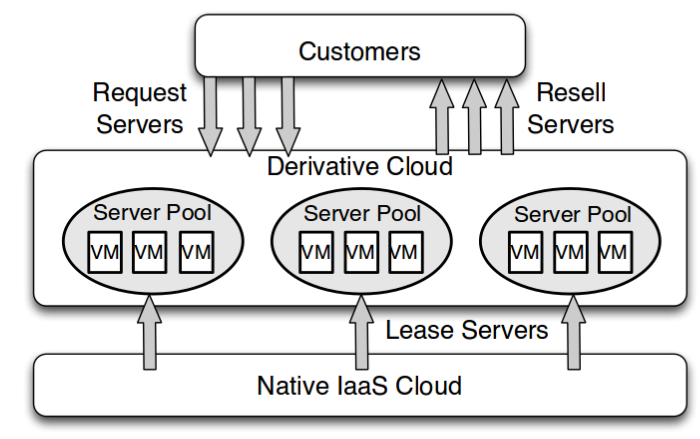
\includegraphics[width=0.7\textwidth]{images/intro/derivative_cloud.png}
      \caption{Depiction of a derivative IaaS cloud platform, Source:\cite{sharma2015spotcheck}}
      \label{img_derivative_cloud}
    \end{figure}

    This idea of deterministic provisioning can be expanded to a \textit{derivative cloud} environment as purposed by P.Sharma in his 
recent work \cite{sharma2015spotcheck} which repackages and resells resources purchased from native IaaS platforms. A derivative cloud can 
offer resources to customers with different pricing models and availability guarantees not provided by native platforms using a mix of 
resources purchased under different contract. Derivative cloud providers rent resources from native cloud providers to resell services to 
customers as shown in Fig:\ref{img_derivative_cloud}.

    Although containers support has been provided in most major operating systems today, it is most popular and widely used in operating 
systems running on a Linux kernel. Our entire work would focus on elastic provisioning of containers in a native Linux environment and 
extend its implications to the derivative setup. However at this stage, we focus on deterministic provisioning of memory and disk-caching 
as a resource in this thesis.

  \section{Memory management in clouds}
  
    Memory as a resource has gained popularity recently with emergence of more memory intensive applications in various fields of 
computing like data analytics, caching that have a very strong correlation with application performance that is dependent on the memory 
available in the system. Most memory sensitive applications constantly use any unused memory available in the system to benefit them. A 
simple example is an Key-value used to cache frequent key's accessed by a web application. 

    Currently available provisioning knobs in the Linux container framework are quite effective while provisioning for applications when 
the host system isn't under any memory pressure and overcommitment (When resources promised on a system is more than resources available). 
However overcommitment is a fundamental requirement to provision cloud servers to maximize provider running costs as discussed earlier. In a 
native Linux system, memory pressure might be generated due to the following 

      \begin{enumerate}
	\item Additional memory required by processes of other containers
	\item More memory required by processes/services running on host Linux OS
	\item Memory pressure generated by kernel threads/processes
      \end{enumerate}
      
      Let's see how memory overcommitment and pressure can disrupt desired functionality of the existing container framework provided by 
Linux containers.

    \subsection{Issues in native container environment}	
    
    Consider two containers provisioned for running Mongo-DB containers from 2 different customers on a same host machines. Now that 
average memory used by the 2 containers are in the ratio of 1:2 and the customers for the 2 containers are also paying for their services in 
the same ratio. Let's call container with 1x workload usage as Mongo-Low and that of with 2x usage as Mongo-High. Now assume the customers 
have been provisioned using existing memory knobs with the same ratio as shown in Tab:\ref{table_initial}. For the sake of simplicity assume 
that all the containers over-provisioned for all other resources and aren't throttled by any other resource. Low and High can be thought of 
relative priorities of each of the containers.
	
	\vspace*{1em}	
	\begin{table}[!h]
	  \begin{center}
	    \begin{tabular}{ l | p{3cm} | p{2.2cm} | p{2.2cm} | p{2.2cm} }	      	    
		  & Average Memory Usage & Cost Paid for Service & Memory Provisioned & Desired Throughput \\ 
	      \hline
	      \hline
	      Mongo-Low  & 1x & 1x & 1x & 1x \\  
	      \hline
	      Mongo-High & 2x & 2x & 2x & 1x \\
		
	    \end{tabular}
	  \caption{Memory Provisioned for the Containers using existing memory provisioning knobs}
	  \label{table_initial}
	  \end{center}	  
	\end{table}
	\vspace*{1em}
	
	\pagebreak
	
	\begin{figure*}[t!]
	  \centering
	  \begin{subfigure}[t]{0.48\textwidth}
	    \centering
	    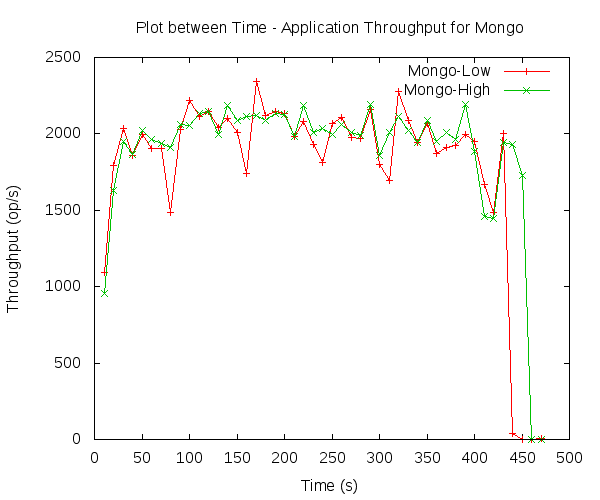
\includegraphics[width=1\textwidth]{images/intro/native.png}
	    \caption{Running applications without containers}
	    \label{plot_intro_native}
	  \end{subfigure}
	  ~ 
	  \begin{subfigure}[t]{0.48\textwidth}
	    \centering
	    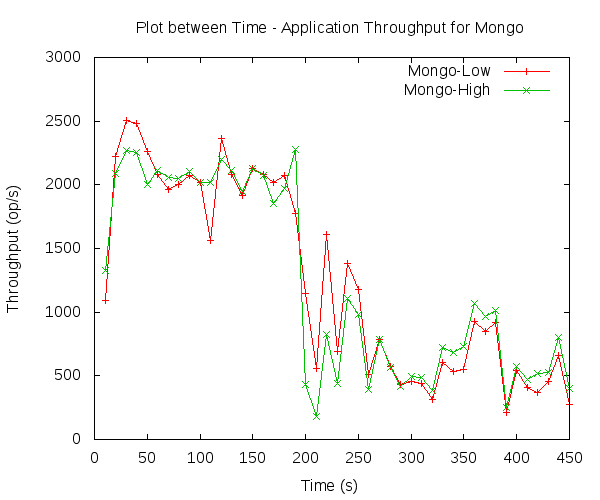
\includegraphics[width=1\textwidth]{images/intro/observed.png}
	    \caption{Observed after provisioning containers using existing knobs}
	    \label{plot_intro_observed}
	  \end{subfigure}
	  ~ 
	  \begin{subfigure}[t]{0.48\textwidth}
	    \centering
	    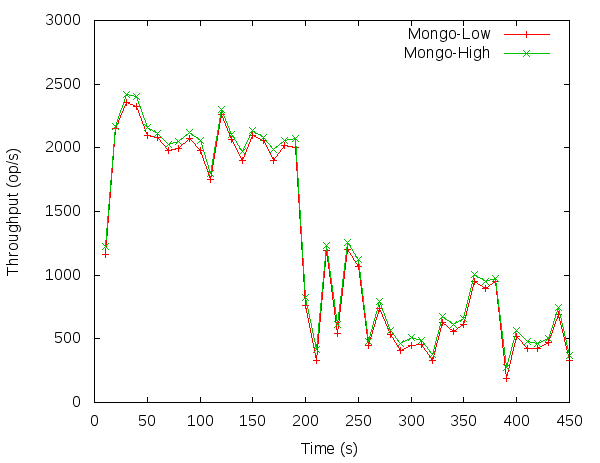
\includegraphics[width=1\textwidth]{images/intro/desired.png}
	    \caption{Desired after provisioning containers using knobs}
	    \label{plot_intro_desired}
	  \end{subfigure}
	  \caption{Application throughputs for problem establishment}
	\end{figure*}
	
	Consider 3 cases as described below. In cases 2 and 3, containers are allowed to run normally for about 100s and there after 
which free memory in the system gradually reduces by generating of memory pressure by an external entity. 
	
	\begin{itemize}
	  \setlist{nosep,after=\vspace{\baselineskip}}
	  \item Case-1: Running applications natively in a system with 1:2 memory assignments and no pressure 
	  \item Case-2: Observed throughputs after provisioning with existing knobs under pressure
	  \item Case-3: Desired throughputs under pressure
	\end{itemize}
	
	Fig:\ref{plot_intro_native} shows the simple case where both the containers achieve desired throughputs when running on a system 
with no container specific provisioning. The containers start execution with no memory pressure and hence must be able to each equal 
throughputs initially in all 3 cases although. Case-2 still shows lower levels of application performance for higher provisioned 
containers even when the system is under no pressure. In observed throughputs under pressure Fig:\ref{plot_intro_observed}, we 
observe that throughputs of Mongo-High (Container with higher priority) is negatively affected at some point or the other, when in reality 
its throughput had to be better if not same as shown in Fig:\ref{plot_intro_desired} considering its higher resource allocations. 
	
	\pagebreak

	\begin{table}
	  \begin{center}
	    \begin{tabular}{ l | c | c | c }	      	    
		  & No Pressure & Observed & Desired \\ 
	      \hline
	      \hline
	      Mongo-Low  & 1825 & 1268 & 1255$-$ \\  
	      \hline
	      Mongo-High & 1972 & 1242 & 1255$+$ \\
		
	    \end{tabular}
	  \caption{Average throughput in each case (op/s)}
	  \label{table_intro_th}
	  \end{center}	  
	\end{table}
	
	Table:\ref{table_intro_th} shows how average throughputs vary in each case. It can be seen that the average throughput in case-2 
which is the provisioning of containers using existing knobs may negatively impact containers with higher allocations. By looking at the 
example here, we can conclude by saying that 
	
	\begin{enumerate}
	  \item Native memory allocations work well with containers where there doesn't exist any memory overcommitment and pressure
	  \item However when the two occur, memory reclamation may adversely affects containers which are better provisioned (since they 
were promised higher QOS) than those which aren't.
	\end{enumerate}
    
    \subsection{Amplification of issues in derivative cloud environment}
      
      Considering the above described setup to derivative cloud where the native cloud provider is using VMs to provision customer demands. 
This VM acquired from the native cloud provider is again repacked and resold by the derivative cloud provider to specific customers. In 
this case, this situation further complicated due to two reasons,
      
      In the native case, memory overcommitment was a required condition for the previously described situation to arise. Consider the case 
where all containers were assigned memory considering the available system memory in such a way that there is no overcommitment, however 
now the native cloud provider (host system) could reduce the memory available to the system using different memory reclamation policies at 
the host.
       
       \begin{enumerate}
	  \item Memory overcommitment is not a required condition
	  \item Memory pressure maybe introduced by three factors described earlier or an additional factor like an external host system 
driver (eg: Balloon Driver)
       \end{enumerate} 

      The reclamation could be trigger by a host driver like the \textit{Balloon Driver} that is widely used by the \textit{Hypervisor} 
(Entity that manages VMs) by cloud providers. This leads to further discrepancies in the memory management at the container level. 
  
  \section{Caching in the cloud}
    Caching of data has played a crucial role in provisioning for applications on the cloud. Caching provides a faster
    mechanism to access frequently accessed data. There are several web services these days that make use of CDNs (content 
    distribution networks) to cache their frequently accessed to minimize response time by spreading these CDNs servers across
    the globe. This is one form of commonly used caching frameworks. Another form of caching occurs at the application level
    where frequently accessed key-value pairs are stored in a key-value store like Redis \cite{redis}, Memcached \cite{memcached}.
    However our work deals with cloud frameworks where the cloud provider caches client data to improve client performance.
    Let's begin with how caching occurs in a traditional cloud setup.
    
   \subsection{Drawbacks of caching in traditional (VM) cloud setup}
      
     \begin{figure}
      \centering
      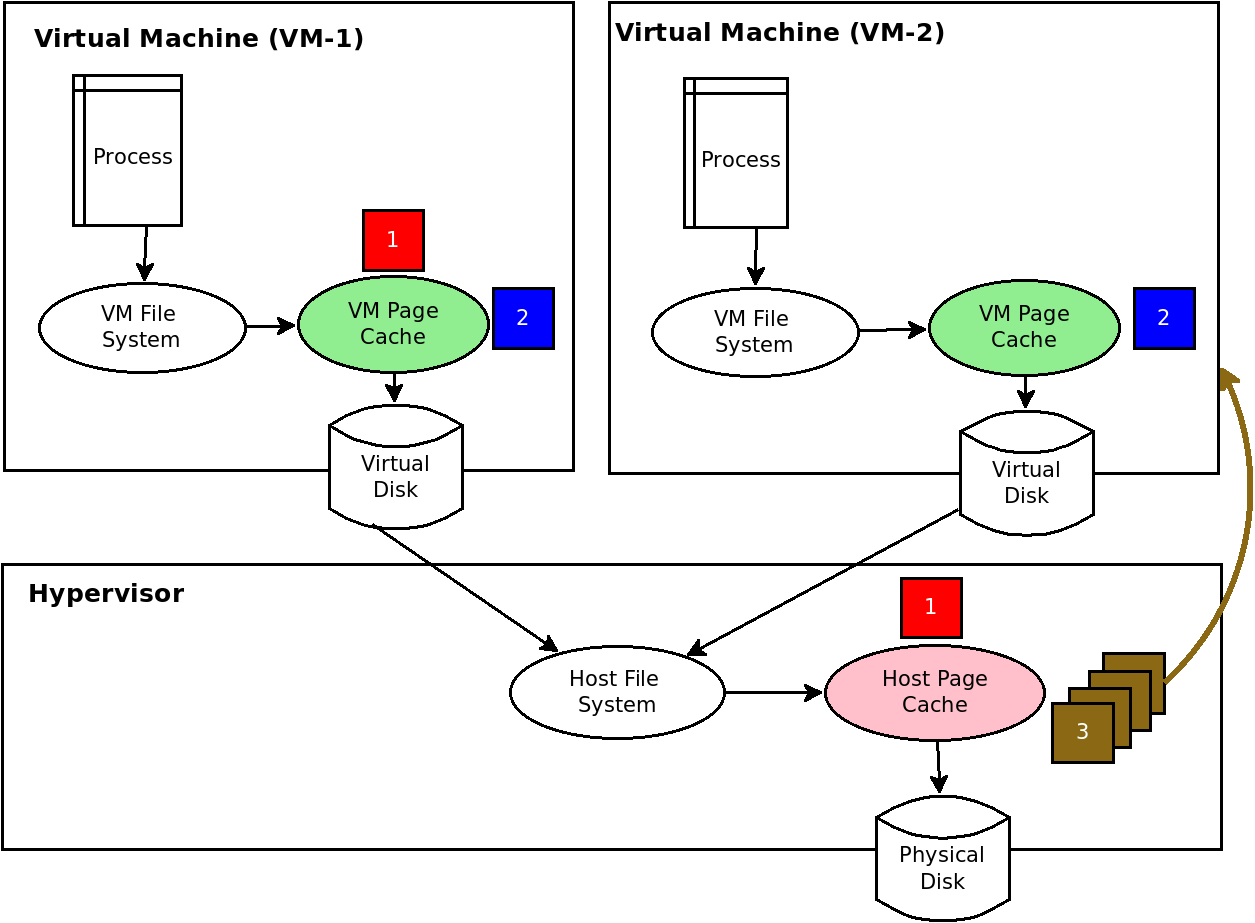
\includegraphics[width=0.8\textwidth]{images/intro/issues_in_hypervisor.png}
      \caption{Drawbacks of caching in traditional VM cloud setup}
      \label{img:drawbacks_traditional}
    \end{figure}
    
    Fig~\ref{img:drawbacks_traditional} depicts a traditional host page caching at occurs in a virtualized setup. There are
    two-levels of caching occurring here, one at the guest and the other at the host level. 
    Both these caches are controlled by their respective operating systems and are unaware of one another.
    This leads to improved performance but will also lead to wastage of resource. 
    The drawbacks of such a setup are (as illustrated in Fig~\ref{img:drawbacks_traditional} listed below,
    
      \begin{enumerate}
	\item A copy of the same page is present at the hypervisor page cache and the VM page cache.
	\item A copy of the same page maybe present across VMs.
	\item The host page cache could be flooded with page caches from a single or a set of VMs.
      \end{enumerate}
      
   \subsection{Hypervisor managed caching}
    
    To overcome above drawbacks, several works\cite{mishra2014comparative, koller2015centaur} have proposed the use of
    a more controlled caching framework called the \textit{Hypervisor managed caches} as depicted in Fig~\ref{img:hc}.  
    Hypervisor managed caches are caching frameworks whose control lies in the hands of the native cloud provider. 
    The native cloud provider cloud provision these caches to satisfy an application level objective which could be 
    exposed as a service to their clients or also to configured based on a global provider level policy to maximize 
    throughput.
    
      \begin{figure}
	\centering
	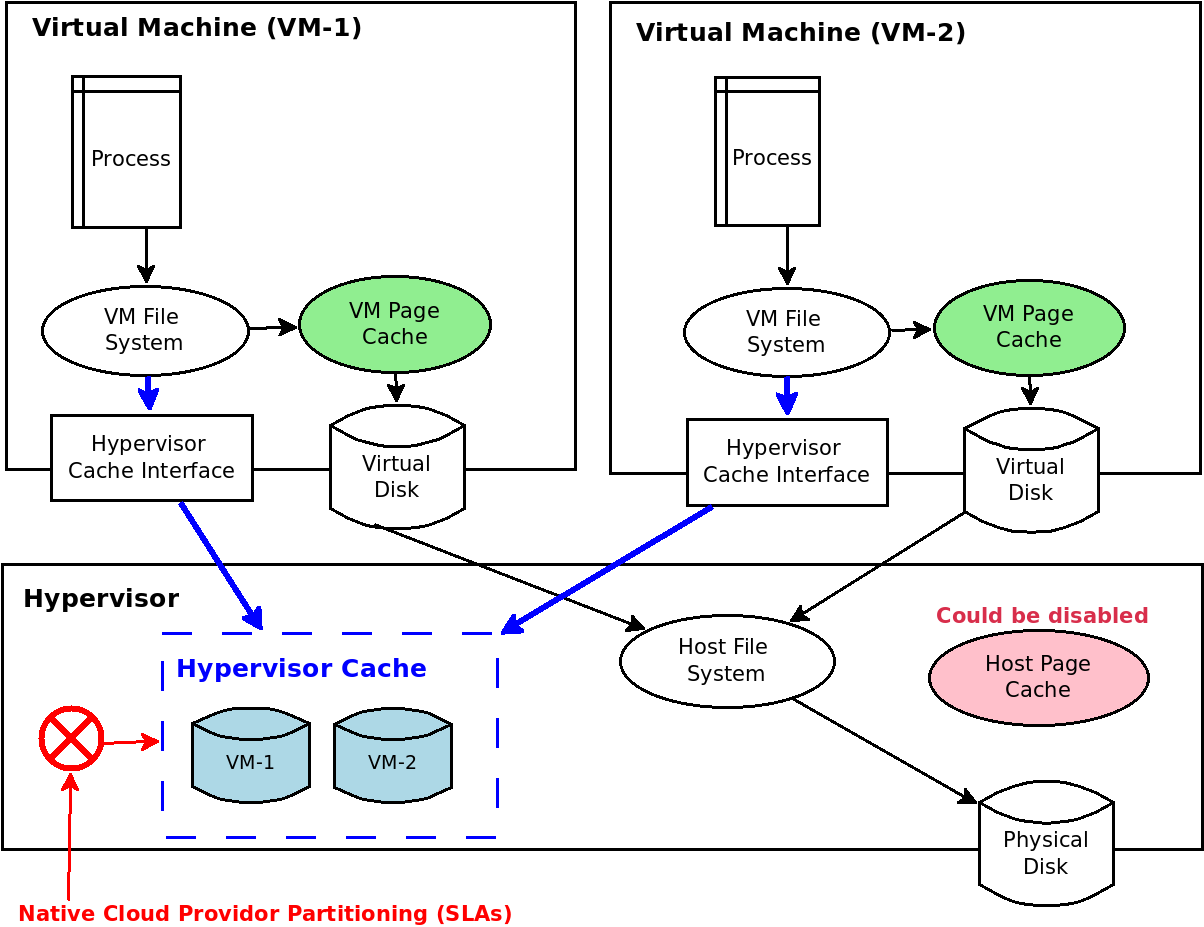
\includegraphics[width=0.8\textwidth]{images/intro/hc.png}
	\caption{Hypervisor managed cache}
	\label{img:hc}
      \end{figure}    
    
    Hypervisor managed caches eliminates the drawbacks previously discussed by providing an exclusive cache there by 
    removing any redundant pages. The cache size can be configured there by eliminating flooding of page cache by a single
    VM. Typically host-side page cache is turned off when hypervisor managed cache is enabled.
    
    \subsection{Issues of caching frameworks in derivative clouds}
      Hypervisor managed caches have shown significant improvements in performance improvements in a native cloud environment, 
      but however when it comes to derivative clouds the existing frameworks aren't able to differentiate the nested levels
      of virtualization entities. Existing cache partitioning frameworks\cite{koller2015centaur, stefanovici2015software}
      that partition caches for each VM assumed a single application running and hence successfully partitions the same, 
      however with multiple applications running in an derivative setup, cache partition to achieve application objectives 
      (SLAs) becomes challenging as shown by \dd{}\cite{doubledecker}. \dd{} was the preliminary work done based on which 
      this work is built upon, however even with \dd{} like other caching frameworks there exist drawbacks as discussed 
      below.
      
      \subsubsection{Lack of framework support in derivative clouds}
	Caching frameworks existing lack support for derivative clouds. They lack the engineering components required to 
	exposed container as an individual provisioning entity. \dd{} addressed this by exposing cache provisioning to a
	derivative cloud provider. A similar approach could be used for other partitioning frameworks as well.
      
      \subsubsection{Dual layers of isolated control}
	With a caching framework like mentioned above incorporated into a derivative cloud setup makes it have two isolated
	control centers - one at the native cloud provider level (hypervisor) and the other at the derivative 
	cloud provider (VM) level. The native cloud provider is only responsible for partitioning the cache, where as the 
	derivative cloud provider is responsible for distributing the VM memory among the container. Such isolation makes
	it difficult for a derivative cloud provider to get a holistic view while provisioning for application objectives. 
	
      \subsubsection{Application cache sensitivity is unaccounted}
	With two levels of memory provisioning - In-VM and hypervisor cache makes it challenging to provision applications 
	has some applications have specific needs of In-VM requirements whereas the others are more flexible about it. 
	Caching frameworks fail to address this issue.
    
  \section{Problem description}  
    Keeping the above drawbacks in mind, the following are the outline of the problem description for our work. 
  
   \subsection{Memory management for containers}
      In the initial phase of our work we wish to 
      \begin{enumerate}
	\item Understand the existing memory management policies used by Linux to manage containers.
	\item Identify issues with existing policies and purpose new policies to be supported for.
	\item Do the same for both native and derivative cloud environments. 
	\item Design a solution to support purposed policies and empirically evaluate its correctness.
      \end{enumerate}

   \subsection{Holistic cache and memory management for containers}
      In this phase of our work we wish to
      \begin{enumerate}
	\item Understand existing cache partitioning frameworks.
	\item Identify issues with the existing frameworks.
	\item Come up with solution to fix identified issues and empirically evaluate its correctness.
      \end{enumerate}

  \section{Contributions}
    The following are the contributions of our work.  
      \begin{enumerate}
	\item Built a differentiated memory management controller for containers. This work has been 
	accepted in \textit{IEEE ICDCS '17} for the poster track.
	\item Designed and implemented an decentralized memory (and cache) management framework for containers. This work 
	is in submission at \textit{ACM Middleware '17}.
      \end{enumerate}

    
  \chapter{Background}

  
  \section{Memory management between processes in Linux}
  
    Memory is allocated/deallocated in terms of pages in any operating system. Memory management in Linux is done using techniques like 
virtual memory, demand paging, swapping caching etc. They separate between the memory needed by a process and the memory physically 
allocated on the RAM. The OS creates a large virtual address space for each process. In this section we focus on how memory is managed 
between processes or a group of processes. We mainly focus on how memory is assigned and reclaimed between them.  
  
    \subsection{Memory pages used by a process}
      Memory used by processes are divided into 2 types of pages	
      \begin{enumerate}	
	\item Anonymous Pages: Pages those which are not associated with any files on disk. They are process memory pages.
	\item Page cache pages: Are an in-memory representation of a part files on the disks.	
	\item Mapped pages: File page with VA mappings
      \end{enumerate}
  
    \subsection{Memory allocation}
      When the process needs memory to be allocated, Linux decides the how this memory is going to be allocated physically on the RAM. The 
process/ application does not see in physical RAM addresses. It only sees virtual addresses from the virtual space assigned to each process.
The OS uses a page file located on the disk to assist with memory requests in addition to the RAM. Less RAM means more pressure on the Page 
file. When the OS tries to find a piece of memory that's not in the RAM, it will try to find in the page file, and in this case they call it 
a page miss. The actual physical memory allocated (RSS) to a process depends on how much free memory is available in the system. On free 
memory becoming freshly available in the system, the OS tries to equally distribute the available memory to all processes that are 
demanding for more memory.

    \subsection{Memory reclamation without container support}
      Two lists 
      
  \section{Containers}
    \subsection{Control groups (Cgroups)}
      \subsubsection{Memory Cgroup}
	\paragraph{Memory reclamation with Cgroups}
      
  
  \section{Caching}
  
   \subsection{Hypervisor managed caching}
      \subsubsection{T-MEM cache}
    
   \subsection{Multilevel caches}
    
   \subsection{Application specific cache partitoning}
      \subsubsection{MRC construction}
      
   \subsection{Double decker: Second chance cache for derivataive clouds}
  
      

       
  
\chapter{Related work}

  There have been several attempts to provide efficient memory management for virtual machines. The most prominent used approach is of 
that Ballooning \cite{waldspurger2002memory}. Ballooning is an mechanism that reclaims pages considered least valuable by the guest OS 
running inside the virtual machine. This allows the VM to decide which memory pages to release instead of the host trying to determine this.
Gerḿan Molt́o \cite{molto2013elastic} expands the idea of Ballooning to provide a system to monitor the VM memory and apply vertical 
elasticity rules in order to dynamically change its memory size by using the memory ballooning technique provided the KVM hypervisor. 
Overdriver \cite{williams2011overdriver} on the other hand presents a system that handles all durations of memory overload. It adapts its 
mitigation strategy to balance the trade offs between migration and cooperative swap to handle memory overcommitments. Ex-Tmem 
\cite{venkatesan2014ex} stores clean pages in a two-level buffering hierarchy with locality-aware data placement and replacement. It 
enables memory-to-memory swapping by using non-volatile memory and eliminates expensive I/O caused by swapping.
  
  Looking at researches that have looked at resource provisioning, CloudScale \cite{shen2011cloudscale} can resolve scaling conflicts 
between applications using migration, and integrates dynamic CPU voltage/frequency scaling to achieve energy savings with minimal effect on 
application SLOs. Tim Dornemanna\cite{dornemann2009demand} proposed a solution that automatically schedules workflow steps to underutilized 
hosts and provides new hosts using cloud computing infrastructures in peak-load. The system was based on BPEL to support on-demand resource 
provisioning. Aneka \cite{calheiros2012aneka}, is a platform for developing scalable applications on the Cloud, that supports provisioning 
resources from different sources and supporting different application models. It support the integration between Desktop Grids and Clouds. 
Elastic Application Container (EAC) \cite{he2012elastic} is a virtual resource unit for delivering better resource efficiency and more 
scalable cloud applications. 

  A derivative cloud is a nested setup, virtual machines nested in virtual machines\cite{williams2012xen} or containers deployed in virtual machine 
  \cite{sharma2015spotcheck, gcp}, the latter being the focus of this work.  

  There has been extensive work carried out in hypervisor caching\cite{lu2007virtual, magenheimer2009transcendent, mishra2014comparative, schopp2006resizing}.
  On top of this there has been work carried out to partition hypervisor caches based on application SLAs \cite{schopp2006resizing, koller2015centaur}.

  Although there are several existing works in elastic resource provisioning (including memory) for virtual machines as listed above. There 
  has been no attempt to provide an deterministic memory management policy for containers. To our knowledge this is our first attempt to do 
  so.
  
  Applicability of hypervisor caching in a derivative cloud setup is hindered due to inability of existing frameworks to support this sort of
  provisioning, and also we would like to look at the overall picture of memory management at all levels of the hierarchy along with the cache
  partitioning to satisfy application SLA. 

%   \subsection{Hypervisor managed caching}
%       \subsubsection{T-MEM cache}
%     
%    \subsection{Multilevel caches}
%     
%    \subsection{Application specific cache partitoning}
%       \subsubsection{MRC construction}
%       
%    
  
\chapter{Differentiated memory management controller for containers}

  The existing memory management controller posses a few issues when it comes to managing memory among containers in an
  over-committed scenario. We initially bring out these issues, and then propose a solution and evaluate our solution
  with respect to the existing controller.
  
  \section{Drawbacks of existing memory management for containers}
  \label{sec:controller_issues}
  
    We have used empirical evaluations to verify and demonstrate our hypotheses. These hypotheses bring out the issues existing container
    memory management controller---Memory \cg{}. We have used both a native cloud testbed and an derivative cloud testbed to establish 
    our issues.
    
    \subsection{Experimental setup}
    
      The following are the experimental setup configurations, metrics and workloads used to establish the correctness of our hypotheses
      in a native cloud environment.
      
       \subsubsection{Experimental configurations}
    
	The set of configurations used for an analysis of memory management techniques in a container environment must be relevant, 
	and easy to apply. The following configurations fit this criteria, and have been used for the evaluation.
	
	\begin{itemize}
	  \item \textbf{Number of containers:} The number of containers that are currently executing in the system.
	  \item \textbf{Memory soft limit of container:} The minimum promised memory to a given container by the system on which the 
    container is executing.
	  \item \textbf{Memory hard limit of container:} The maximum memory that can be assigned to a container by the system on which the 
    container is executing.
	  \item \textbf{Memory usage of each container:} The usage of a container at a given point in time, that is generated by the workload 
    executing inside the container.
	  \item \textbf{Workload:} The workload that is running inside each of the container. Workloads can vary based on the type of operation 
    they perform, the ratio of anonymous memory pages they consume to that of page cache pages.  
	  \item \textbf{External memory pressure:} The memory pressure that is generated in the system in order to reduce the free memory 
    available in the system and trigger memory reclamation. This pressure could be either generated by a process on the same system / driver 
    that is running in the host system.
	  \item \textbf{Size of machine:} Size of Machine refers to the maximum memory available in the system inside which all the 
    containers are executing.      
	\end{itemize}  
      
      \subsubsection{Metrics of interest}
      
	The following are the metrics of interest to us that would help us analyze the experiments.
	  
	    \begin{enumerate}
	    \item \textbf{Memory assigned to each container:} Total memory assigned to a container at any given instant
	    \item \textbf{Soft memory reclaimed for each container:} Memory reclaimed from each container using SMR
	    \item \textbf{Total memory reclaimed for each container:} Total Memory reclaimed from container (SMR + GLR)
	    \item \textbf{Memory reclaimed using GLR:} Memory reclaimed from all containers and other processes running on system using GLR
	    \item \textbf{Memory reassigned for each container:} Memory reassigned to each container on freeing up of memory
	    \item \textbf{Application specific metrics:} Application metrics of the workload running inside containers like throughput, total 
    time taken etc.
	    \end{enumerate}
      
      \subsubsection{Workloads}
      
	This section presents the list of workloads that we have used as primary candidates to evaluate our empirical evaluations. All 
    workloads are chosen keeping in mind the memory intensive nature of the requirement.  
	
	These are the list of Synthetic workloads we have used to establish our problem.
	  
	  \myparagraph{Stress}
	    Stress \cite{stress} is a deliberately simple workload generator for POSIX systems. It imposes a configurable amount of CPU, 
    memory, I/O, and disk stress on the system. It is written in C and has been developed by people at Harvard university. 
	  
	  \myparagraph{Memory hogger}
	    Memory Hogger is a simple C program that allocates an array of specified memory using a simple \texttt{malloc()} and repeatedly 
    writes to these array locations. This only consumes anonymous memory pages.
	  
	  \myparagraph{File hogger}
	    File Hogger is a simple python program that creates a file with specified size and repeatedly updates it line by line there by 
    consuming both anonymous pages and file backed pages.

	These are the list of real workloads we have used to show how the existing problems affect real work applications.
	  
	  \myparagraph{MongoDB}
	    MongoDB \cite{Mongodb} is an open-source, document database designed for ease of development and scaling. Classified as a NoSQL 
    database program, MongoDB avoids the traditional table-based relational database structure in favor of JSON-like documents with dynamic 
    schema. It follows a memory hungry approach where it tries to use up most of system and it actually leaves it up to the OS's VMM to tell it 
    to release the memory.

	\myparagraph{Redis}
	    Redis \cite{redis} is a in-memory data structure store, used as database, cache and message broker. It is used to store a large 
    number of in-memory key-value pairs. Its in-memory nature makes it a prime candidate to use it as a workload in our empirical evaluations.
      
	\myparagraph{YCSB benchmark}
	    We use YCSB \cite{cooper2010benchmarking} (Yahoo Cloud Server Benchmark) project as the benchmark to generate the clients evaluate 
    to the performance of our real workloads i.e MongoDB and Redis servers. The goal of YSCB is to develop performance comparisons of the new 
    generation of cloud data serving systems. It is a framework and common set of workloads for evaluating the performance of different 
    “key-value” stores.
    
  
    \subsection{Issues in native environment}
    
      We have tried to show the issues in container memory management using empirical analysis. We have taken our hypothesis/questions, 
      and mapped them to various experiments to illustrate the issues. Inferences were drawn based on the observations in the experiments. 
    
      \begin{figure}
	\centering
	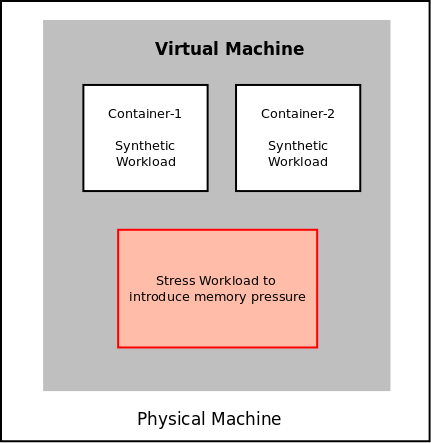
\includegraphics[width=0.5\textwidth]{images/controller_issues/native_testbed.png}
	\caption{Native container testbed}
	\label{img:native_setup}
      \end{figure}
      
       The native testbed consisted of running containers inside a host machine (running inside VM in our case) in complete isolation from 
the external environment as shown in Fig~\ref{img:derived_setup}. This setup which involved a native container testbed, was used to 
understand the existing memory reclamations and establish the problem in a native system using \textbf{synthetic workloads}.
	
      \subsubsection{Host}
	
	\begin{enumerate}
	  \item Intel Core i5-4430 processor @ 3.00GHz
	  \item 4 cores of CPU (with hyper threading support)
	  \item 1 TB of hard disk space
	  \item 8 GB RAM
	  \item Ubuntu 14.04 LTS desktop, 64 bit 
	  \item Kernel version 4.5
	  \item KVM Hypervisor
	\end{enumerate}
      
      \subsubsection{Guest}
	
	\begin{enumerate}
	  \item 3 cores of CPU (with hyper threading support)
	  \item 20 GB of virtual disk space
	  \item 2-6 GB RAM (based on experimental configuration)
	  \item Ubuntu 16.04 LTS desktop, 64 bit
	  \item Kernel version 4.7
	  \item Container technology: Docker
	\end{enumerate}
	
      Memory Hogger and File Hogger were used to generate the memory pressure inside the containers. External pressure was generated 
using Stress workload running directly on the host machine.
  
  
      The configuration in Table~\ref{table_native_base} is the base configuration for all experiments in this section. Any changes the base 
      configuration has been mentioned in the procedure of each of the experiment.

	\begin{table}	 
	  \begin{center}
	    \begin{tabular}{ l | c | c }
	      & Container-1 (M1) & Container-2 (M2) \\ 
	      \hline
	      \hline
	      Size of VM & \multicolumn{2}{c}{2 GB} \\	      
	      \hline
	      Workload & Memory Hogger & Memory Hogger \\
	      \hline
	      Hard Limit & 1000 MB & 1000 MB \\  
	      \hline
	      Soft Limit & 150 MB & 150 MB \\  
	      \hline
	      Memory Usage & 500 MB & 500 MB \\
	      \hline
	      Exceed & 350 MB & 350 MB \\
	      \hline 
	      External Pressure & \multicolumn{2}{l}{ 200 - 400 - 600 - 800 - 1000 MB} \\
	    \end{tabular}	    
	    \caption{Base configuration for native container experimentation}
	    \label{table_native_base}
	  \end{center}
	\end{table}
	
      Most experiments involved setting up of 2 containers. Workloads were used to introduce system memory pressure from containers. At 
      this point there was no memory pressure in the system (free memory was still available). Now the external pressure using Stress was 
      introduced after about 20s which created memory pressure in the system that triggered reclamation. The external pressure kept on increasing 
      by 200 MB in intervals of 40s. Each interval had a gap of 10s for memory to be reassigned to containers.
      
      \subsubsection{Reclamation above soft limits}
      
	\myparagraph{Hypothesis} 
	  Hypothesis to be verified,
	  \begin{enumerate}
	    \item Majority of reclamation when containers exceed occurs using SMR (Soft Memory Reclamation) 
	    \item SMR purely based on exceed value of the container
	    \item Containers that exceed equally are iteratively targeted
	  \end{enumerate} 
	  
	  \myparagraph{Procedure}
	    To demonstrate the correctness of our hypothesis we the base configuration described in Table~\ref{table_native_base} and change 
  the usage to 700 MB and soft limit to 350 MB there by simulating an scenario (Exp-1) where \textbf{Both containers exceeded by the same 
  values}.
	  
	  \begin{figure*}[t!]
	    \centering
	    \begin{subfigure}[t]{0.48\textwidth}
	      \centering
	      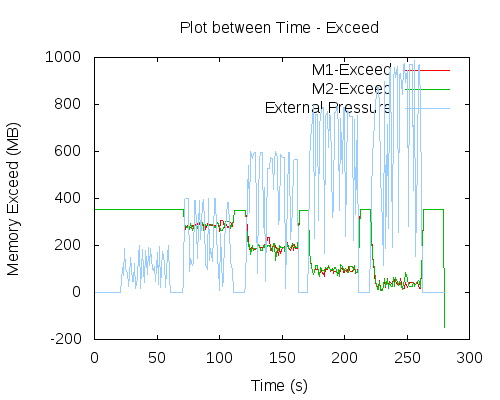
\includegraphics[width=1\textwidth]{images/controller_issues/exceed_only/Exceed.png}
	      \caption{Memory exceed plot}
	      \label{img_exceed_only_1_exceed}
	    \end{subfigure}
	    ~ 
	    \begin{subfigure}[t]{0.48\textwidth}
	      \centering
	      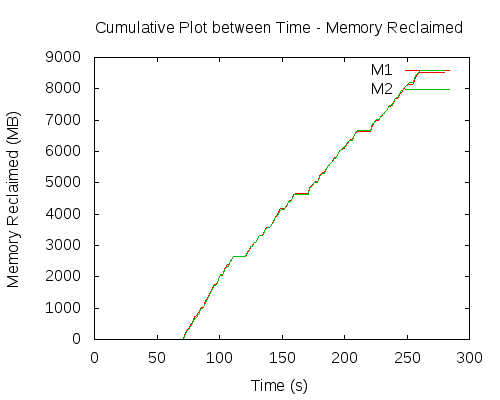
\includegraphics[width=1\textwidth]{images/controller_issues/exceed_only/Memory_Reclaimed.png}
	      \caption{Cumulative soft memory reclaimed plot}
	      \label{img_exceed_only_1_smr}
	    \end{subfigure}
	    ~ 
	    \begin{subfigure}[t]{0.48\textwidth}
	      \centering
	      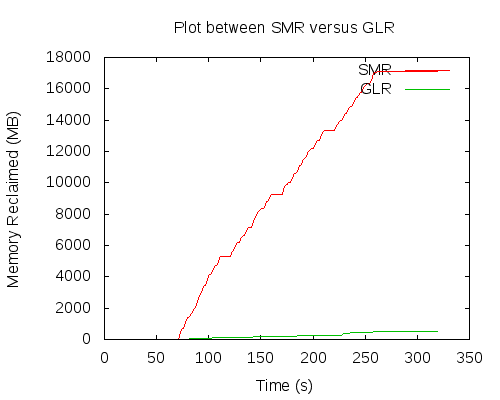
\includegraphics[width=1\textwidth]{images/controller_issues/exceed_only/compare.png}
	      \caption{SMR versus GLR}
	    \label{img_exceed_only_1_compare}
	    \end{subfigure}
	    \caption{Plots for analysis of reclamation when both containers are exceeding by same value}
	  \end{figure*}
	  
	  \myparagraph{Observations}
	    The following are the observations,
	    \begin{itemize}
	      \item As seen from Fig~\ref{img_exceed_only_1_exceed}, Fig~\ref{img_exceed_only_1_smr} - memory reclaimed from containers 
  iteratively from one after the other as their exceeds are same.
	      \item Fig~\ref{img_exceed_only_1_compare} shows how most reclamation when containers exceed occurs using SMR however it is seen 
  that there is minimum reclamation occurring using GLR as well.
	    \end{itemize}

	  \myparagraph{Inference}	
	    The following are the inferences,
	    \begin{itemize}
	      \item SMR is purely based on exceed value.
	      \item Most reclamation when containers exceed occurs using SMR, however the GLR kicks in every reclamation request to evict any 
  inactive page cache pages in the system (may/may not belong to container).
	      \item Containers that exceed equally are iteratively target for reclamation one after the other.
	    \end{itemize}
      
      \subsubsection{Reclamation below soft limits}
      
      \myparagraph{Hypothesis}
	Does our hypotheses of reclamation below soft limits falling back to native system reclamation hold good ?
	
      \myparagraph{Procedure}  
	To test the reclamation patterns in containers below soft limits, we created containers as mentioned in Table~\ref{table_native_base} 
  and changed soft limits (Exp-2) of both containers to 1000 MB there by making the current \textbf{usage of both containers below soft 
  limits}. We used hooks in the kernel code to track requests satisfied by soft memory reclamation (SMR) and global LRU based reclamation 
  (GLR).
	
	\begin{figure*}[t!]
	    \centering
	    \begin{subfigure}[t]{0.48\textwidth}
	      \centering
	      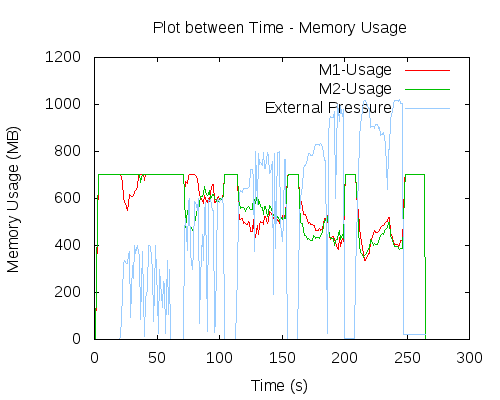
\includegraphics[width=1\textwidth]{images/controller_issues/global_lru/mu.png}
	      \caption{Memory Usage Plot}
	      \label{img_no_sl_mu}
	    \end{subfigure}
	    ~ 
	    \begin{subfigure}[t]{0.48\textwidth}
	      \centering
	      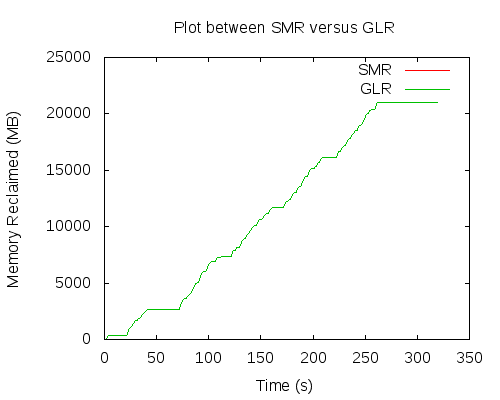
\includegraphics[width=1\textwidth]{images/controller_issues/global_lru/compare.png}
	      \caption{SMR versus GLR Plot}
	      \label{img_no_sl_global_vs_local}
	    \end{subfigure}
	    \caption{Plots for when both containers are having same usage but no exceeds}
	  \end{figure*}
	
	\myparagraph{Observations}
	  The following are the observations.
	  \begin{itemize}
	    \item As seen from Fig~\ref{img_no_sl_mu}, there is no hand-in-hand reclamation that occurs to containers below their soft 
  limits although the containers are running the same workload, unlike hand in hand reclamation that occurs in memory usage above soft limits.
	    \item Since both containers are below SL, all reclamation is occurring using the GLR (Global LRU based reclamation) as seen by 
  Fig~\ref{img_no_sl_global_vs_local}
	  \end{itemize}

	\myparagraph{Inferences}
	  The following are the inferences.
	  \begin{itemize}
	    \item Containers with memory usage below soft limits reclamation falls back to native system GLR.
	    \item Reclamation using GLR is haphazard and there is no control over it. 
	  \end{itemize}
   
     \subsubsection{Effect of workloads characteristics on reclamation}
      
	\myparagraph{Question}
	Questions of our interest,
	    \begin{enumerate}
	      \item Effect of workload characteristics on reclamation
	      \item How much of memory is reclaimed from a container in a single reclamation SMR request ?
	    \end{enumerate}
	  
	  \myparagraph{Procedure}
	    We took our base configuration as described in Table~\ref{table_native_base}. However we ran two workloads in this case - Memory 
  Hogger (Exp-4a) and File Hogger (Exp-4b) workloads on it as native theory suggests that containers with page cache pages might be 
  victimized at larger the way it occurs with GLR.	
	  

	  \begin{figure*}[t!]
	    \centering
	    \begin{subfigure}[t]{0.48\textwidth}
	      \centering
	      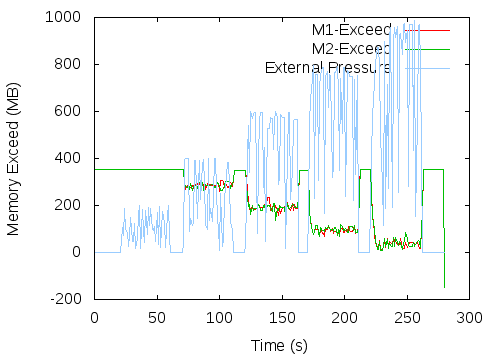
\includegraphics[width=1\textwidth]{images/controller_issues/workload/1/Exceed.png}
	      \caption{Exceed plot for memory hogger}
	      \label{img:workload_1_exceed}
	    \end{subfigure}
	    ~ 
	    \begin{subfigure}[t]{0.48\textwidth}
	      \centering
	      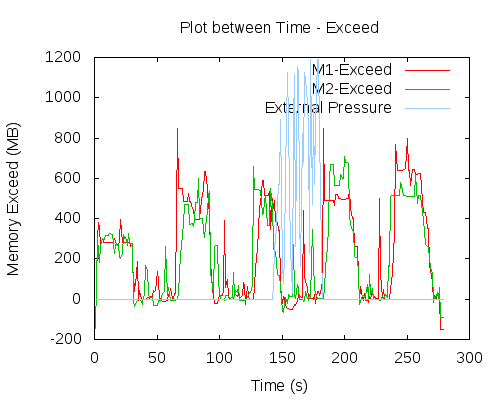
\includegraphics[width=1\textwidth]{images/controller_issues/workload/2/Exceed.png}
	      \caption{Exceed plot for file hogger}
	      \label{img:workload_2_exceed}
	    \end{subfigure}
	    \caption{Plots for analyzing effect of workloads characteristics on reclamation}
	  \end{figure*}		
	    
	  \myparagraph{Observations}
	  The following were the observations,	  
	  \begin{itemize}
	    \item The exceed goes hand in hand as expected but with larger deviation in Fig~\ref{img:workload_1_exceed} and 
  Fig~\ref{img:workload_2_exceed}
	    \item The larger deviation can be accounted to larger reclamation chunks in workloads that have page cache pages similar to how 
  reclamation targets page cache pages in native system
	    \item Further empirical analysis of the reclamation chucks gave us the reclamation chucks to be 
		\begin{center}
		    Reclamation chuck = Anonymous memory pages (\textless 25MB) + Page cache pages
		\end{center}
		In both cases pages from inactive zones were reclaimed before trying to reclaim from active lists.
	  \end{itemize}

	  \myparagraph{Inference}
	    Workloads with page cache pages are reclaimed at larger chunks per SMR request
	  
      \subsubsection{Key Implications}
      \label{sec:mem_management}
    
	Here are the list of key implications that were derivative from running the above experiments in an synthetic environment. We have 
    classified it based on the scenarios as discussed earlier.
	
	\begin{enumerate}
	  \item When containers usage are above soft limits most reclamation occurs using SMR, however the GLR kicks in every reclamation 
    request to evict any  inactive page cache pages in the system (may/may not belong to container).      
	  \item SMR is purely based on exceed value of a container.
	  \item Workloads with page cache pages are reclaimed at larger chunks per SMR request
	  \item Containers with memory usage below soft limits reclamation falls back to native system GLR.
	  \item Reclamation using GLR is haphazard and there is no control over it. 
	\end{enumerate}
	
  
    \subsection{Amplification of issue in derivative clouds}
    
      The following experiment tries to establish the implications of previously established inferences, as to how these affect 
applications running on a derived cloud environment.

      \subsubsection{Testbed}
      \label{sec:derivative_testbed}

      The derivative cloud testbed consisted of running server containers inside a virtual machine (VM-1) which was running on top of a 
physical host machine. Another virtual machine (VM-2) was used to generate clients who connected to servers containers running inside VM-1 
as shown in Fig~\ref{img:derived_setup}. This setup was used to understand the impact of existing memory reclamation patterns on real 
workloads running on a derivative cloud setting.
      
      \begin{figure}
	\centering
	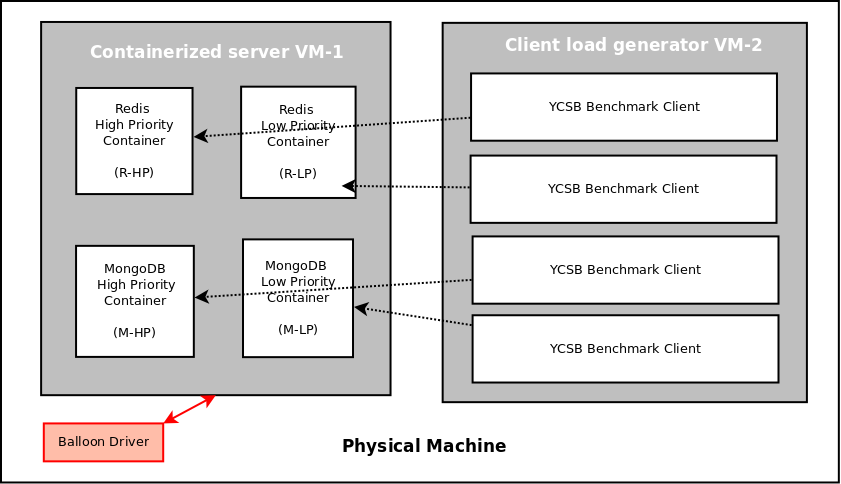
\includegraphics[width=1\textwidth]{images/controller_issues/derivative_setup.png}
	\caption{Derivative cloud testbed}
	\label{img:derived_setup}
      \end{figure}
      
      \paragraph{Host}	
	\begin{enumerate}
	  \item Intel Xeon E5507 @ 2.27GHz
	  \item 8 cores of CPU (with hyper-threading support)
	  \item 125 GB of attached storage, Unlimited NFS attached storage 
	  \item 24 GB RAM
	  \item Ubuntu 14.04 LTS server, 64 bit 
	  \item Kernel version 3.13
	  \item KVM Hypervisor with memory ballooning enabled
	  \item Guest machines were connected using a software bridge
	\end{enumerate}
      
      \myparagraph{Guest}
	The two VMs used in this setup are described here.
	
	\noindent \textbf{VM-1:} Running server containers
	\begin{enumerate}
	  \item 6 cores of pinned CPUs (with hyper threading support)
	  \item 175 GB of virtual disk space (Storage was provisioned using NFS)
	  \item 16 GB RAM
	  \item Ubuntu 16.04 LTS desktop, 64 bit
	  \item Kernel version 4.7
	  \item Container technology: Docker
	  \item Containers inside guest were multiplexed using NAT forwarding
	\end{enumerate}
	
	\noindent \textbf{VM-2:} Running clients that connect to server containers
	\begin{enumerate}
	  \item 1 core of pinned CPU (with hyper threading support)
	  \item 20 GB of virtual disk space (Storage was provisioned using NFS)
	  \item 6 GB RAM
	  \item Ubuntu 16.04 LTS desktop, 64 bit
	  \item Kernel version 4.7
	\end{enumerate}
	
	Redis and MongoDB was used to generate the memory pressure inside the containers. External pressure was generated by varying guest 
balloon size triggered from the host.

      
    \subsubsection{Experimental Flow}
      
      To establish the limitations of nesting-agnostic memory reclamation we performed
      the following experiments. Two Linux+KVM virtual machines were used, one in a nesting setup,
      which hosted containers, the second generated workloads for the 
      container-hosted applications. The nested VM was provisioning with 6 vCPUs
      and 16 GB memory and the workload generating VM has allocated 1 vcPU and 6 GB memory.
      The nesting setup consisted of four Docker containers~\cite{docker}
      which executed with \redis{}~\cite{redis} and
      \mongo{}~\cite{Mongodb} workloads. 
      Default configurations of the applications executed within
      the contains is as shown in Table~\ref{tbl:table_default_config}.
      %The four containers consisted of 2 containers running Redis \cite{redis} and MongoDB \cite{mongodb} workloads each. 
      The YSCB~\cite{cooper2010benchmarking} workbench was used to generate workload datasets and 
      as a workload generator. For the first 100 seconds the applications were executed without 
      memory pressure to consume as much memory as required. Beyond 100 seconds, memory pressure
      was generated from the host and memory from the nested VM reclaimed at rate of 2 GB
      every 30 seconds.

      \begin{table}[t]
	  \begin{center}	   
	    \begin{tabular}{| l | c | c | c | c |}
	      \hline
	      Container & \hl{} (GB) & \sol{} (GB) & \# of records & Usage (GB)  \\ 
	      \hline
	      \hline
	      Redis-Low & 2 & 0.5 & 500K & 1.3 \\  
	      \hline
	      Redis-High & 4 & 1 & 1000K & 2.6 \\  
	      \hline
	      Mongo-Low & 2 & 0.5 & 500K & 1.3 \\
	      \hline
	      Mongo-High & 4 & 1 & 1000K & 2.6 \\
	      \hline
	    \end{tabular}	  
	  \end{center}
	  \caption{Default configuration of the four application containers running in the derivative cloud setup}
	  \label{tbl:table_default_config}	  
	\end{table}
    
     \subsubsection{Impact in derivative environment}
     \label{sec:drawback_env}
	
      \begin{figure*}
	      \begin{subfigure}{0.48\textwidth}
      %	  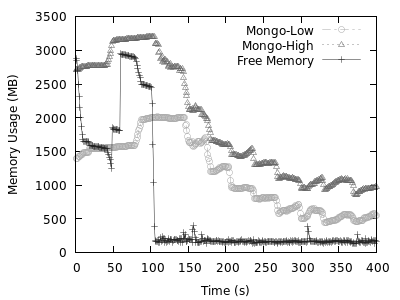
\includegraphics[scale=0.44]{images/inference/memory_usage_mongo.png}
		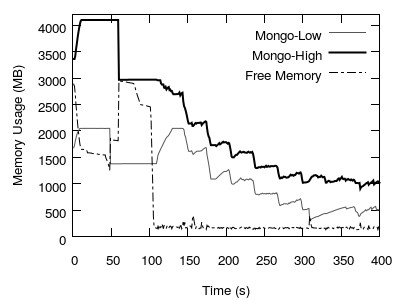
\includegraphics[width=\textwidth]{images/controller_issues/derivative_issues/memory_usage_redis.png}
		\caption{\footnotesize Memory usage for \redis{} applications.}
		\label{plot_inference_redis}
	      \end{subfigure}
	      \begin{subfigure}{0.48\textwidth}
		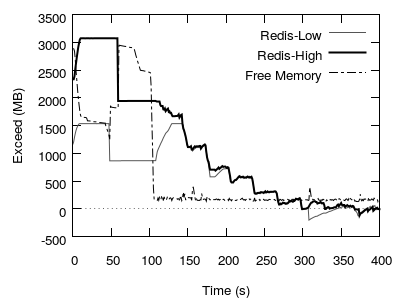
\includegraphics[width=\textwidth]{images/controller_issues/derivative_issues/exceed_redis.png}
		\caption{\footnotesize Extent of memory usage exceed for \redis{} applications.}
		\label{plot_exceed_redis}
	      \end{subfigure}
	    \begin{subfigure}{0.48\textwidth}
      %	  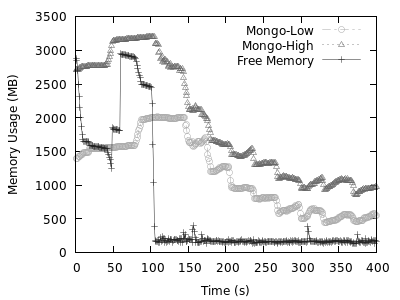
\includegraphics[scale=0.44]{images/inference/memory_usage_mongo.png}
		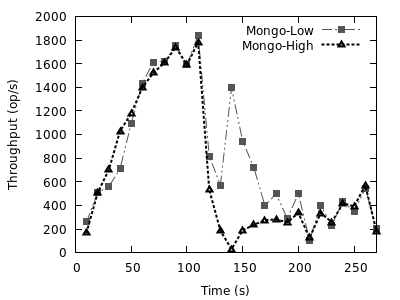
\includegraphics[width=\textwidth]{images/controller_issues/derivative_issues/mongo_throughput.png}
		\caption{\footnotesize Impact of improper memory allocations on \mongo{} applications.}
		\label{plot_throughput_mongo}
	      \end{subfigure}
	      \begin{subfigure}{0.48\textwidth}
		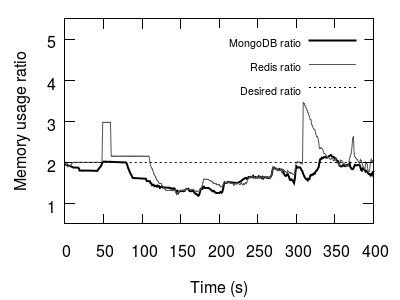
\includegraphics[width=\textwidth]{images/controller_issues/derivative_issues/memory_ratio.png}
		\caption{\footnotesize Memory allocation ratios.}
		\label{plot_inference_ratio}
	      \end{subfigure}
      \caption{Plots illustrating limitations in maintaining memory ratios in derivative clouds}
      \end{figure*}
      
      Figure~\ref{plot_inference_redis} shows the memory consumed by the 
      containers executing the two \redis{} workloads and free memory 
      available in the virtual machine.
      The two containers are configured to consume memory in the ratio of 1:2
      (refer to Table~\ref{tbl:table_default_config}), via \hl{} and \sol{}
      specifications. At 50 seconds, both the \redis{} workloads, which
      are already at their \hl{}, try to allocate more memory, this results
      in container-specific memory reclamation---the free memory in the
      system increases and the memory usage of the two containers drops
      to 1.35 GB and 2.7 GB.
      At 100 seconds, the hypervisor-based balloon controllers starting
      exerting memory pressure---demanding 2 GB every 30 seconds.
      As shown in Figure~\ref{plot_inference_redis}.
      just after 100 seconds, the free memory in the system drastically drops.
      The extent of memory \emph{exceed} beyond 
      the \sol{} specifications is shown in Figure~\ref{plot_exceed_redis}.
      Since, the \redis-high application exceeds by a large extent (2 GB more
      that \sol), the cg{} subsystem penalizes this container for 
      reclamation.
      Further, due
      to the free memory available, and reduced memory consumption of the 
      \redis-high workload, the usage for the \redis-low application 
      increases for an epoch and just before 150 seconds, the extent
      of exceed beyond the \sol{} specifications for both the containers
      is similar. \emph{Note that this is how the cg{} subsystem operates,
      it penalizes the container with the maximum extent of exceed, till
      all of them exceed by the same absolute value and then 
      penalizes them equally.} This process essentially does not
      adhere to the memory usage ratios that were expected with the
      \sol{} and \hl{} specifications. Figure~\ref{plot_inference_ratio}
      shows the memory usage of the \redis{} and \mongo{} applications,
      which drops below the 1:2 ratio from 100 seconds to 300 seconds.
      At 300 seconds, the extent of exceed decreases to zero and
      the system switches to the global reclamation (GLR) mode.
      Beyond this point, the memory reclaimed is not container-agnostic
      and variable ratios of usages are observed.
    
    \subsection{Key Implications}
    The key takeaways from these experiment are as follows,
      \begin{itemize}
      \item Memory reclamation uses the extent of exceeded usage above a containers \sol{}.
      Containers with higher exceed values are penalized to a larger extent.
      \item The Linux cg{} systems attempts to maintain similar extent of exceed for
      memory usage during reclamation when all container are above their \sol's.
      %Reclamation is based on exceed values of each container when any of the containers are using more memory than their SLs. Containers with higher exceed values will be penalized more. Reclamation falls back to host LRU based reclamation without considering container provisioning when memory usage of every containers are below their SLs. Can user provide/ensure priority to a container over other containers using existing memory control knobs (SL and HL)?
      % \item Reclamation falls back to host LRU based reclamation without considering container provisioning when memory usage of every containers are below their SLs. %Priority definition on the basis of SL and HL will become useless if exceed of all containers are zero.
      % Can we define priority of containers using SL and HL?
      \item A per-container \sol{} and \hl{} specification does not guarantee proportionate
      memory allocation during memory pressure situations.
      %Soft Limit is not a definite guarantee, it is mere best effort approach. Can we ensure SL as a definite guarantee to higher priority container(s), if possible?
      \end{itemize}
      This Linux \cg{} reclamation policy does not accommodate different user-specified policies
      that are desired---proportionate memory usages at all instances,
      order-of-reclamation across containers etc. This is especially required in nested
      hosting environments where derivative service provides would be benefited
      by providing a rich set of prioratization features.
    
  \section{Requirements for a new memory management controller}
  
    We wish to build an updated memory management controller that is controller aware, and is able to enforce a differential management
    policy by a native or derivative cloud provider. The following are the list of requirements of policies that we would like to enforce
    using this controller,
  
    \begin{enumerate}
      \item \textbf{Prioritized memory allocation:} Currently the notion of priority doesn't exist in container specific memory allocation 
although the notion of priority exists in other resources. The existing knobs fail to enforce priority used to manage memory in containers. 
      \item \textbf{Deterministic provisioning:} The policy to be designed must eliminate existing non determinism that exists while 
managing memory between containers in existing system.
      \item \textbf{Elastic provisioning:} Memory allocated must be re-sizable as and when required. 
      \item \textbf{Adaptive:} On changing resources provisioned to the system as in the case of an derivative environment, the policy 
enforced must still do it's best in maintaining promised QOS.
      \item \textbf{Differentiated memory reclamation:} The policy could build around the notion of differentiated memory reclamation when 
the system falls under memory pressure.
      \item \textbf{Strict enforcement of limits:} The notion of hard and soft limits that exist must be strengthened.      
    \end{enumerate}
    
  We would like to design a new controller keeping the above requirements in mind.
   
  
  \section{Proposed memory management controller}
      
      Enforcing memory allocation proportions across containers when no memory pressure exists is possible with the soft-limit and hard-limit 
      configuration parameters. However, as discussed in Section~\ref{sec:controller_issues}, these knobs do not provide deterministic memory 
      provisioning when the system is under memory pressure. As part of this work, we design for two new policies to provide deterministic 
      memory provisioning in nested setups under memory pressure
      
      \subsection{Controller logic}
	When the VM in which the containers are executing comes under memory pressure, memory is reclaimed using the container specific LRU lists 
	(as SMR) as well as the Global LRU list (as GLR) by the guest operating system.
	Memory reclamation depends on the extent of \textit{exceed} in memory usage above the specified \sol---estimated as the difference 
	in the two values. 
	The container having a higher \textit{exceed} is victimized during memory pressure first.
	We redefine this notion of \textit{exceed} with one that is based on proportionality weight of each container. 
	The proportional allocation of a container is the ratio of the container weight to the total weight across all containers in a 
	VM multiplied by the total memory usage across all containers (Equation~\ref{eqn:pa}). The proportionate \textit{exceed} value is the 
	difference of the container's proportional memory allocation and its current usage (Equation~\ref{eqn:ex}). 
	Finally, the memory reclamation policy is modified to target the container having  the highest proportionate \textit{exceed} value for each
	reclamation request. Similar to the default reclamation policy, the global LRU list for reclamation is used once memory usage 
	of all containers is below \sol{} specifications.
	
	\small
	\begin{align}
	  T\_U &= \sum_{i=1}^{n}U_{i} \\
	  T\_W &= \sum_{i=1}^{n}W_{i} \\
	  PA_{i} &= T\_U \times (\frac{W_{i}}{T\_W}) \label{eqn:pa}\\
	  EX_{i} &= U_{i} - PA_{i} \label{eqn:ex}
	\end{align}

	\footnotesize
	\textit{
	\\
	U$_{i}$: Memory usage of i$^{th}$ container \\
	W$_{i}$: Relative weight of i$^{th}$ container \\
	T\_U: Total memory usage by all containers \\
	T\_W: Summation of relative weights of all containers \\
	PA$_{i}$: Proportional memory allocation of i$^{th}$  container \\
	EX$_{i}$: Proportionate exceed value of i$^{th}$ container
	}
	\normalsize
    
      \subsection{Policies supported by our controller}
      
	The following are the policies enforceable by our controller.  
	
	\subsubsection{Policy 1: Proportionate memory allocation}
	  This policy aims to ensure that all memory allocated to container is based on relative weights specified as configuration parameters.
	  The proportional memory allocation is enforced during situations of memory pressure and during no pressure. For example, consider 
	  two containers with an intended proportionate memory allocation in the ratio 1:2. Further, assume that their \sol{} values are set 
	  to 1 GB and 2 GB, respectively, and their current usage is 2 GB and 4 GB respectively.
	  With a memory reclamation demand of 1 GB, most of the memory will be reclaimed from the container with the larger extent of usage, 
	  since the extent of exceed is 2 GB as compared to 1 GB of the smaller container. The resulting usages after reclamation will be 2 GB 
	  and 3 GB, respectively, violating the proportionate ratio of 1:2. The proposed proportionate allocation policy aims to maintain 
	  the 1:2 ratio in all memory pressure situations.
	
	\subsubsection{Policy 2: Application-specific differentiated allocation}
	\label{sec:memory_distribution}
	  This policy provides the flexibility of providing specific rules and or categories to application containers, e.g. gold, silver,
	  bronze etc. Containers mapped to each of these categories have different reclamation rules or the categories themselves can 
	  imply an ordering for reclamation.
  
  \section{Modifications made to Linux memory Cgroup}
      
      We modify memory Linux \cg{} memory management subsystem to conform to the polices specified earlier. We have made
      three major changes to this subsystem as described below.
     
    
    \subsection{Per container configurable weights}
      A new per-cgroup state variable is introduced to specify a \emph{weight}
      parameter for each container and is also
      exposed through \texttt{sysfs} interface for every container.
      These weights enforce a notion of priority among containers; 
      higher the weight for a container the higher its priority and proportion.
      The relative ratio of the weights, dictate the proportion of memory allocation.
      Cloud providers can modify these weights in the derivative setup 
      (also applicable to native cloud providers using 
      containers for provisioning) to enforce priority among containers 
      executing within VMs.
    
    \subsection{Flexible reclamation size}
      The current soft-memory reclamation policy (SMR), targets one container and 
      reclaims a non-deterministic amount of memory from it for every 
      request. The extent of reclamation depends on the anonymous region (from which
      a fixed size is reclaimed) and the disk page cache (from which a large
      portion is reclaimed). Since the page cache size is non-deterministic,
      reclamation extent can also be non-deterministic.
      This may lead to a container being targeted exclusively for a particular 
      reclamation request, leading to large deviations 
      from weighted allocations. To overcome this issue, we have 
      capped reclamation chunk size to a maximum of 50 MB. 
    
    \subsection{Deterministic reclamation}
      As part of the Linux \cg{} memory reclamation process, soft-reclamation (SMR)
      reclaims memory from each container till memory usage is above the
      \sol specification. Simultaneously, a small amount of memory is also
      reclaimed from the system-wide pool of pages (GLR). In our solution,
      to maximize deterministic reclamation we perform proportionate
      reclamation across containers till the usage of containers reduces
      to zero. Beyond this situation, the system-wide global LRU list is
      used for further reclamations.
      Since the SMR policy is container-aware, this strategy
      provides us a better handle over memory provisioning for containers. 
    
  
  \section{Empirical evaluation of our controller}
       
    We show the effectiveness of our approach empirically in this section. Experimental set-up for the most part remains same as that 
mentioned in Section~\ref{sec:derivative_testbed}. Any changes to the set-up is mentioned in the respective subsections.

    Experiments are performed with the same workload and set-up except for the size of VM-1. At the beginning of the experiment, size of VM-1 
is 20 GB which is gradually reduced to 3.5 GB, at the rate of 1.5 GB every 20s (started at 50s). Relative memory weights for the \mongo{} 
containers are in the ratio of 1:2 (1 for low and 2 for high priority containers) as are the relative weights for the \redis{} 
containers. These weights are added using the newly added \textit{weight} parameter in the memory \textit{Cgroup}. 

% \begin{figure}
% 	  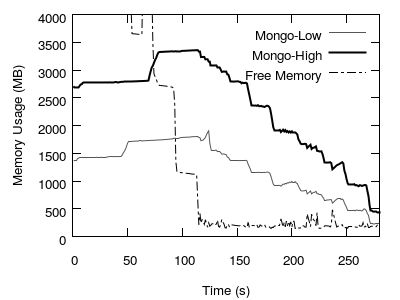
\includegraphics[scale=0.45]{images/mem_sol/sl=hl_mtp/memory_usage.png}
% 	  \caption{\footnotesize Memory usage by Mongodb containers when SL=HL, using modified controller}
% 	  \label{mem_sol_sl=hl_mongo}
% \end{figure}
% 	~
% \begin{figure}
% 	  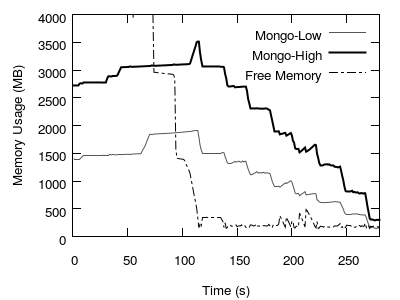
\includegraphics[scale=0.45]{images/mem_sol/sl!=hl_mtp/memory_usage.png}
% 	  \caption{\footnotesize Memory usage by Mongodb containers when SL!=HL, using modified controller}
% 	  \label{mem_sol_sl!=hl_mongo}
% \end{figure}	
	

\begin{figure*}
	\begin{subfigure}{0.30\textwidth}
	  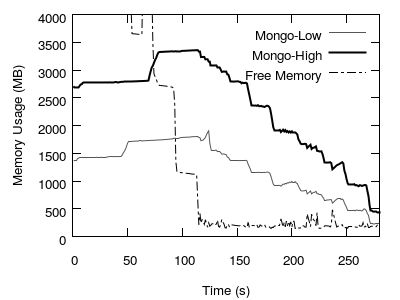
\includegraphics[scale=0.4]{images/mem_sol/sl=hl_mtp/memory_usage.png}
	  \caption{\footnotesize Memory usage by Mongodb containers when SL=HL}
	  \label{mem_sol_sl=hl_mongo}
	\end{subfigure}
	~
	\begin{subfigure}{0.30\textwidth}
	  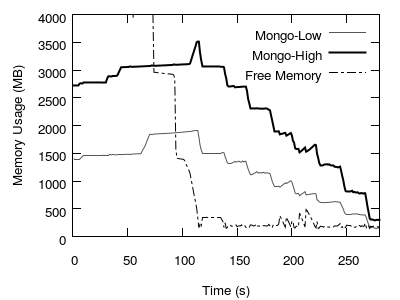
\includegraphics[scale=0.4]{images/mem_sol/sl!=hl_mtp/memory_usage.png}
	  \caption{\footnotesize Memory usage by Mongodb containers when SL$\neq$HL}
	  \label{mem_sol_sl!=hl_mongo}
	\end{subfigure}	
	~
	\begin{subfigure}{0.30\textwidth}
	  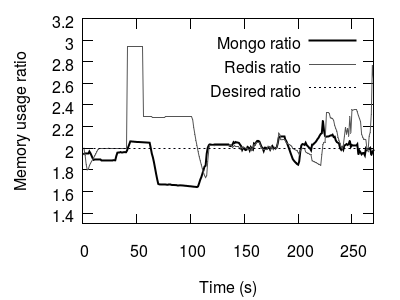
\includegraphics[scale=0.4]{images/mem_sol/memory_ratio_base.png}
	  \caption{\footnotesize Memory usage ratios between MongoDB and Redis containers}
	  \label{mem_sol_ratios}
	\end{subfigure}
	~
	\begin{subfigure}{0.5\textwidth}
	  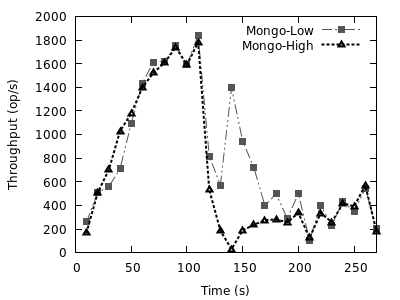
\includegraphics[scale=0.6]{images/mem_sol/mongo_before.png}
	  \caption{\footnotesize Application throughputs with existing memory controller}
	  \label{throughput_mongo_before}
	\end{subfigure}
	~
	\begin{subfigure}{0.5\textwidth}
	  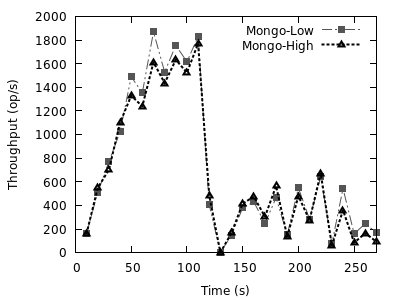
\includegraphics[scale=0.6]{images/mem_sol/mongo_after.png}
	  \caption{\footnotesize Application throughputs with modified memory controller}
	  \label{throughput_mongo_after}
	\end{subfigure}	
  \label{fig:mem_sol}
\caption{Impact of modified controller on low and high priority containers}
\end{figure*}

  
    \subsection{Effectiveness of our controller}
    
      We have tested the effectiveness of our approach in both cases: (i) Soft Limit is equal to Hard Limit (SL=HL) and (ii) Soft Limit is not 
equal to Hard  Limit (SL$\neq$HL), because memory reclamation methods for both cases are different as mentioned in Section~\ref{sec:mem_management}. 

Figure \ref{mem_sol_sl=hl_mongo} and Figure \ref{mem_sol_sl!=hl_mongo} depicts the memory usage patterns for \mongodb{} containers for cases 
(i) and (ii) respectively. We observe a gradual decrease in memory allocated to the low and high priority containers in both cases once the 
system runs out of free memory at about 120 seconds. The ratios of memory allocated to containers can be seen to be in accordance with
their relative weights, unlike the earlier case when there is no modified controller.
We observed similar pattern in case of \redis{} container. 
%However unlike the earlier case (without our modified controller), the memory allocated to containers are in the ratios according to their relative weights. Similar pattern is also observed for Redis containers. 
This pattern of relative memory allocations can be observed more prominently when comparing Figure \ref{plot_inference_ratio} and Figure \ref{mem_sol_ratios} 
which shows memory usage ratios between low and high priority containers (closer to 2, the better) using existing controller and our 
modified controller respectively.

The effect of better memory allocation is notable in the application throughputs. The existing controller produces better throughputs 
for the lower priority \mongodb{} containers in the interval 100-200s as seen in Figure \ref{throughput_mongo_before}. With our modified 
controller, both the low priority and high priority containers produce similar throughput as seen in Figure \ref{throughput_mongo_after}. 
The similar throughputs observed are strongly connected to the fact that low and high priority containers are provisioned with 1:2 memory 
allocations and so are the ratio between their usage patterns (Provisioning is done to avoid contention due to any other resource). Similar 
throughput impacts are also observed with \redis{} containers. Hence credit share not only produces better memory allocations, but also 
enhances application performance for containers.
    
    \subsection{Differential QOS containers}
    
      Consider the application specific differentiated allocation policy specified in Section 
\ref{sec:memory_distribution} where we would like to prioritize a container from being 
victimized. Let's call this container as a gold container. We have used same set-up 
(SL$\neq$HL) to test this. We have prioritized the gold container using the higher weights 
(Weights of the order of $10^{3}$ relatively higher) to avoid reclamation from it unless it's necessary.
There are also other containers running inside the VM with lower QOS and let's call them silver containers.

In Figure \ref{priority_cont} we have plotted only the memory usage for the gold and one silver container for ease of analysis. We 
observe that at about 120 seconds free memory drops and the reclamation kicks in. Victimization of gold container is much lesser than other 
containers until the other containers usage near zero. This shows how we could use our weighted controller to enforce differential 
service QOS containers.

\begin{figure}
  \centering
  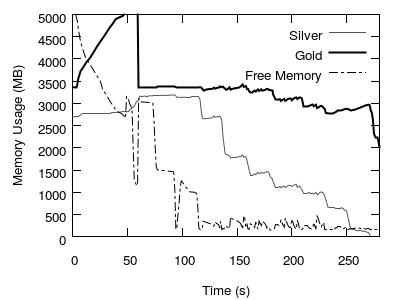
\includegraphics[scale=0.6]{images/mem_sol/gold/memory_usage.png}
  \caption{Memory usage plot showing implication of relative weights provide differential QOS guarantees}
  \label{priority_cont}
\end{figure}
    
    \subsection{Impact of reclamation chunk size}
    
    
    The native reclamation method has no notion of limit on the
amount of memory that can be reclaimed from a targeted container. This leads to larger 
reclamation amounts from a container thereby deviating it from the desired relative 
allocations.

Figure \ref{mem_ratio} shows the ratio of memory usage between \mongodb{} containers for default (native) case and reclamation
chunk size of 50 MB. We consider observation after 120 seconds, as that is when the pressure kicks in and triggers 
reclamation. Although the 50 MB capping of reclamation chunk provides better memory ratios than the default case most of
the time, it still deviates from desired behavior in the interval 180-220 seconds as seen in Figure~\ref{mem_ratio}. 

With smaller maximum reclamation size, we will have finer control over the memory allocation ratios, but this 
comes at the cost of frequent updation. Further investigation has to be done to fix upon a reasonable size to 
maintain balance between performance and precision here. For now, the reclamation chunk size is parameterized in our implementation and can 
be easily modified using a kernel module to alter the maximum reclamation chunk size. We have used reclamation chunk size of 50 MB in our 
implementation and this applies to all the experiments that we have run with our modified controller.

\begin{figure}
  \centering
  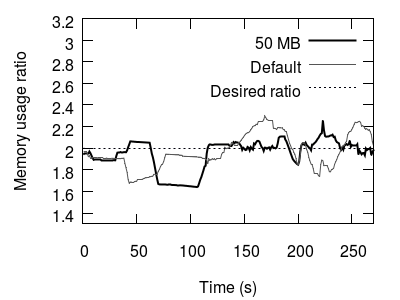
\includegraphics[scale=0.6]{images/mem_sol/memory_ratio.png}
  \caption{Memory usage ratio with different reclamation chunk size}
  \label{mem_ratio}
\end{figure}
  \chapter{Memory management framework for derivative clouds}
  
  Our objective here is to provide a memory management framework for derivative clouds. 
  In order to achieve the same we start off with understanding existing memory management 
  and cache partitioning frameworks. We analyzed them to come up their drawbacks while 
  provisioning for a derivative cloud setup. We made updates to an previous caching partitioning
  framework to make it a more full pledged memory management framework than just a cache partitioning
  framework. My initial work involved understanding the existing infrastructure and come up with
  drawbacks and make updates to the design to accommodate the downfalls. We came up with a revised 
  design and implemented the same. We tested it for correctness and empirically evaluated it as well.
  
  \section{Drawbacks of existing framework}
    The following section tries to bring out the drawbacks of existing hypervisor cache partitioning 
    frameworks and how fail to satisfy application SLA requirements. We demonstrate how an two-level
    exclusive (either level-1 or level-2) cache partitioning framework could fail to satisfy requirements 
    and an intermediate partitioning framework would be desirable.
    
    \subsection{Experimental setup}
    \label{sec:dd_setup}
	
      The following section describes the experimental setup used to establish issues, verify correctness and evaluate our 
      solution. Any changes made to the below setup, shall be mentioned beforehand.
      
      \myparagraph{Testbed}	
	Our testbed consists of a single VM, single container running on top of our hybrid implementation of Double decker as shown 
	in Fig~\ref{img:correctness_testbed}. The hypervisor used is KVM, and the container manager used is LXC.  
	
	
	\noindent The physical machine configuration used is as described below,
	  \begin{enumerate}
	   \item Intel(R) Core(TM) i7-3770 CPU @ 3.40GHz
	   \item 4 CPU cores (with multi-threading)
	   \item 8 GB of physical RAM
	   \item 120 GB SSD disk
	  \end{enumerate}

	
	\begin{figure}
	  \centering
	  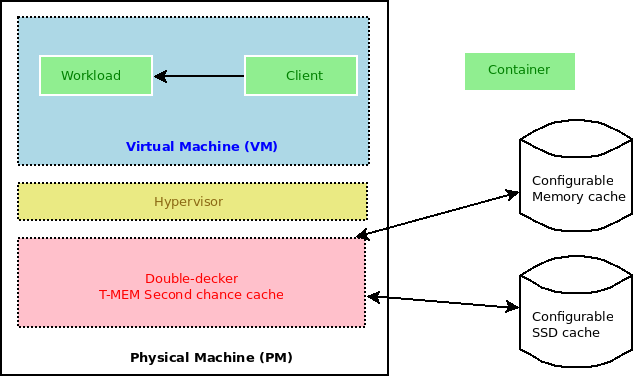
\includegraphics[width=0.9\textwidth]{images/correctness/exp_setup.png}
	  \caption{Experimental testbed for checking correctness}
	  \label{img:correctness_testbed}
	\end{figure}
	
      \subsubsection{Experimental configurations}	
	The set of configurations used for an analysis of memory management framework for a derivative environment 
	must be relevant, and easy to apply. The following configurations
fit this criteria, and have been used for the evaluation.

	  \begin{itemize}
	   \item \textbf{Memory Requirement:} Memory requirement of each container, the estimated total memory used by a container.
	   
	   \item \textbf{Container memory limit:} Size of memory allocated to a container at the Cgroup level (soft and hard limits). 
	   \item \textbf{Memory cache limit:} Size of memory (L1) cache assigned to a container. 
	   \item \textbf{SSD cache limit:} Size of SSD (L2) cache assigned to a container.
	   
	   \item \textbf{Workload:} Workload application that is running inside each of the container. 
	   \item \textbf{Number of containers:} Number of containers that are currently executing in the system.
	   \item \textbf{Number of VMs:} Number of virtual machines that are currently executing in the system.
	  \end{itemize}	  
	  
	  For the sake of simplicity in the evaluations of correctness of our setup. We have only considered a single container, single VM setup 
	  which makes use of synthetic workload to stress our system.
	
      \subsubsection{Metrics of interest}	
	The following are the metrics of interest that would help us establish the correctness of our implementation.
	  
	  \begin{itemize}
	   
	   \item \textbf{Container memory usage:} Guest memory usage of the container.
	   \item \textbf{Memory cache usage:} Memory cache used by the container.
	   \item \textbf{SSD cache usage:} SSD cache used by the container.
	   
	   \item \textbf{Demoted:} Objects moved from memory to SSD cache.
	   \item \textbf{Promoted:} Objects moved from SSD to memory cache.
	   
	  \end{itemize}	  
	  
	  The following metrics are collected both for memory and SSD cache
	  
	  \begin{itemize}
	   
	   \item \textbf{Puts:} Number of objects successfully put into this container cache.
	   \item \textbf{Gets:} Number of objects successfully got from this container cache.
	   \item \textbf{Flushes:} Number of objects flushed from this container cache.
	   \item \textbf{Evicts:} Number of objects evicted from this container cache.
	   
	  \end{itemize}
    
      \subsubsection{Workloads}
      
	This section presents the list of workloads that we have used as primary candidates to evaluate our empirical evaluations. All 
    workloads are chosen keeping in mind the memory intensive nature of the requirement.  
	
	These are the list of workloads we have used to establish issues and evaluate our framework.
	  
	  \myparagraph{Synthetic workload}
	    A self generated synthetic workload generated using \texttt{cat} command that outputs the 
	    content of a file onto \texttt{/dev/null}
	  
	  \myparagraph{MongoDB}
	    MongoDB \cite{Mongodb} is an open-source, document database designed for ease of development and scaling. Classified as a NoSQL 
    database program, MongoDB avoids the traditional table-based relational database structure in favor of JSON-like documents with dynamic 
    schema. It follows a memory hungry approach where it tries to use up most of system and it actually leaves it up to the OS's VMM to tell it 
    to release the memory.

	  \myparagraph{Redis}
	    Redis \cite{Redis} is a in-memory data structure store, used as database, cache and message broker. It is used to store a large 
    number of in-memory key-value pairs. Its in-memory nature makes it a prime candidate to use it as a workload in our empirical evaluations.
      
	  \myparagraph{MySQL}
	    MySQL \cite{mysql} is a database workload that uses anonymous pages to configure its own user-space data cache. 
	    
	  \myparagraph{Filebench}
	    Filebench \cite{filebench} is a synthetic workload used to generate workload patterns of different applications. In filebench we made
	    use of the webserver workload to simulate a webserver.
	  
      
	  \myparagraph{YCSB benchmark}
	    We use YCSB \cite{cooper2010benchmarking} (Yahoo Cloud Server Benchmark) project as the benchmark to generate the clients evaluate 
    to the performance of our real workloads i.e MongoDB, Redis and MySQL servers. The goal of YSCB is to develop performance comparisons of the new 
    generation of cloud data serving systems. It is a framework and common set of workloads for evaluating the performance of different 
    “key-value” stores.
  
    \subsection{Provisioning of caches at different levels based on application requirements}
      Previous results using \dd{}\cite{doubledecker} have shown that certain application requirements 
      (along with their configurations) could be satisfied better by provisioning on a cache of certain 
      performance guarantees. In the previous work\cite{doubledecker} it was shown how an application like 
      Mail-server could be better provisioned on the level-2 (SSD) cache, as its requirement involved 
      having a large WSS (working set size) with slow access rates. On contrary it also showed by cache sensitive 
      applications like the Web-server workload had to be provisioned onto the level-1 (memory) cache. 
      Now let's see if this setup of an exclusive two level cache provisioning schema would satisfy application
      specific need in all cases.
	
	\subsubsection{Inadequate exclusive two level cache provisioning}
	  Consider the following scenario to demonstrate the short comings of the existing exclusive two level cache
	  provisioning framework. Consider the case of a container running web-server workload
	  with a WSS to provisioned onto the hypervisor cache with  no-free memory to be further allocated 
	  at the guest VM and the hypervisor cache available is 0.5 GB at level-1 (Memory) and 1 GB at 
	  level-2 (SSD). Consider a Web-server workload where the desired application throughput is 7000 op/s.
	  
	  \begin{figure}
	    \centering
	    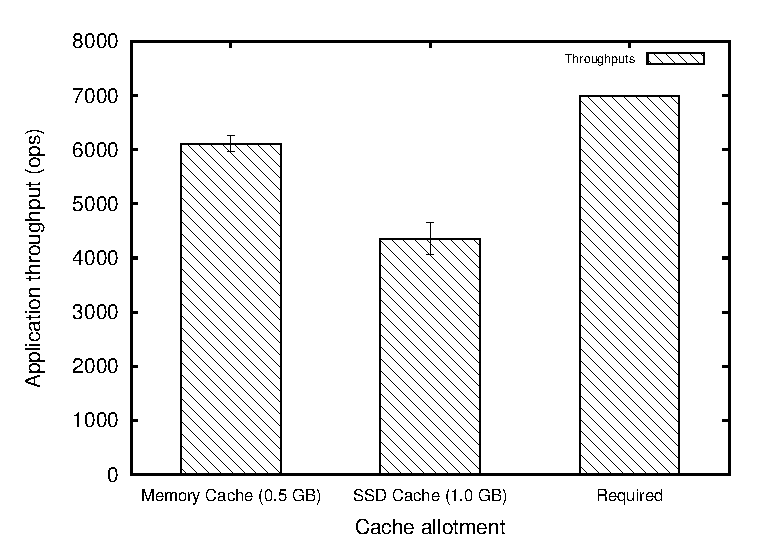
\includegraphics[scale=0.8]{images/dd_hybrid_motivation/throughput.eps}
	    \caption{Inadequate exclusive two level cache provisioning framework}
	    \label{plot:dd_hybrid_motivation}
	  \end{figure}
	  
	  Using our existing double decker cache, we can at max provision at 6000 op/s using memory cache of 0.5 GB as 
	  shown in Fig~\ref{plot:dd_hybrid_motivation}. But say our requirement was beyond that at 7000 op/s. Is there a 
	  workaround to satisfy this requirement ? Could we come up with a better design to satisfy this configuration ?
	  
    
    \section{Cache partitioning framework support for anonymous memory applications} 
	
	\begin{figure}
	  \centering
	  \includegraphics[scale=0.8]{images/dd_decentrailze_motivation/throughput.eps}
	  \caption{Split of memory allocation ratios (In-VM:Cache) to affect application performance}
	  \label{plot:dd_decentrailze_motivation}
	\end{figure}
	
	Application memory requirement is vastly classified into two types - \textit{anonymous and disk backed}.
	Application that require disk backed memory pages can be satisfied be either provisioning them at the 
	VM(guest) memory or at the hypervisor cache. This effect is seen in Fig~\ref{plot:dd_decentrailze_motivation}
	where the memory requirement is split in ratios of in-VM:cache allocations. The plot shows how applications like
	Web-server and \mongo{} which require disk backed pages can be satisfied either in-VM or at the hypervisor cache.
	Kindly note that the application performance is nearly constant in all cases of both these applications as the 
	in-VM memory and the hypervisor cache operate at similar speeds in this case, and had there been difference in
	operational speeds, we would have observed degradation in application performance when moving from left to right 
	in the plot.
	
	Now, if you look at applications like \redis{} and MySQL, their performance is highly affected while provisioning
	them on cache, as they heavily depend on anonymous memory allocated to them (especially Redis). Hence such applications
	need to be provisioned at the guest, however existing cache partitioning frameworks 
	\cite{koller2015centaur, schopp2006resizing} can provision for disk backed workloads fail to address the needs of 
	anonymous memory hungry workloads.
          

  \section{Rethink of existing design}
    
    Keeping the above drawbacks in mind, we re-design the existing differentiated derivative cloud cache partitioning
    framework that \dd{} is and make it more of a memory management framework. There are two crucial ideas around which
    the design is centered around,
    
    \begin{enumerate}
      \item Decentralized memory management framework
      \item Hybrid two-level configurable caches
    \end{enumerate}
    
    \noindent These two components are discussed below.
  
    \begin{figure}
      \centering
      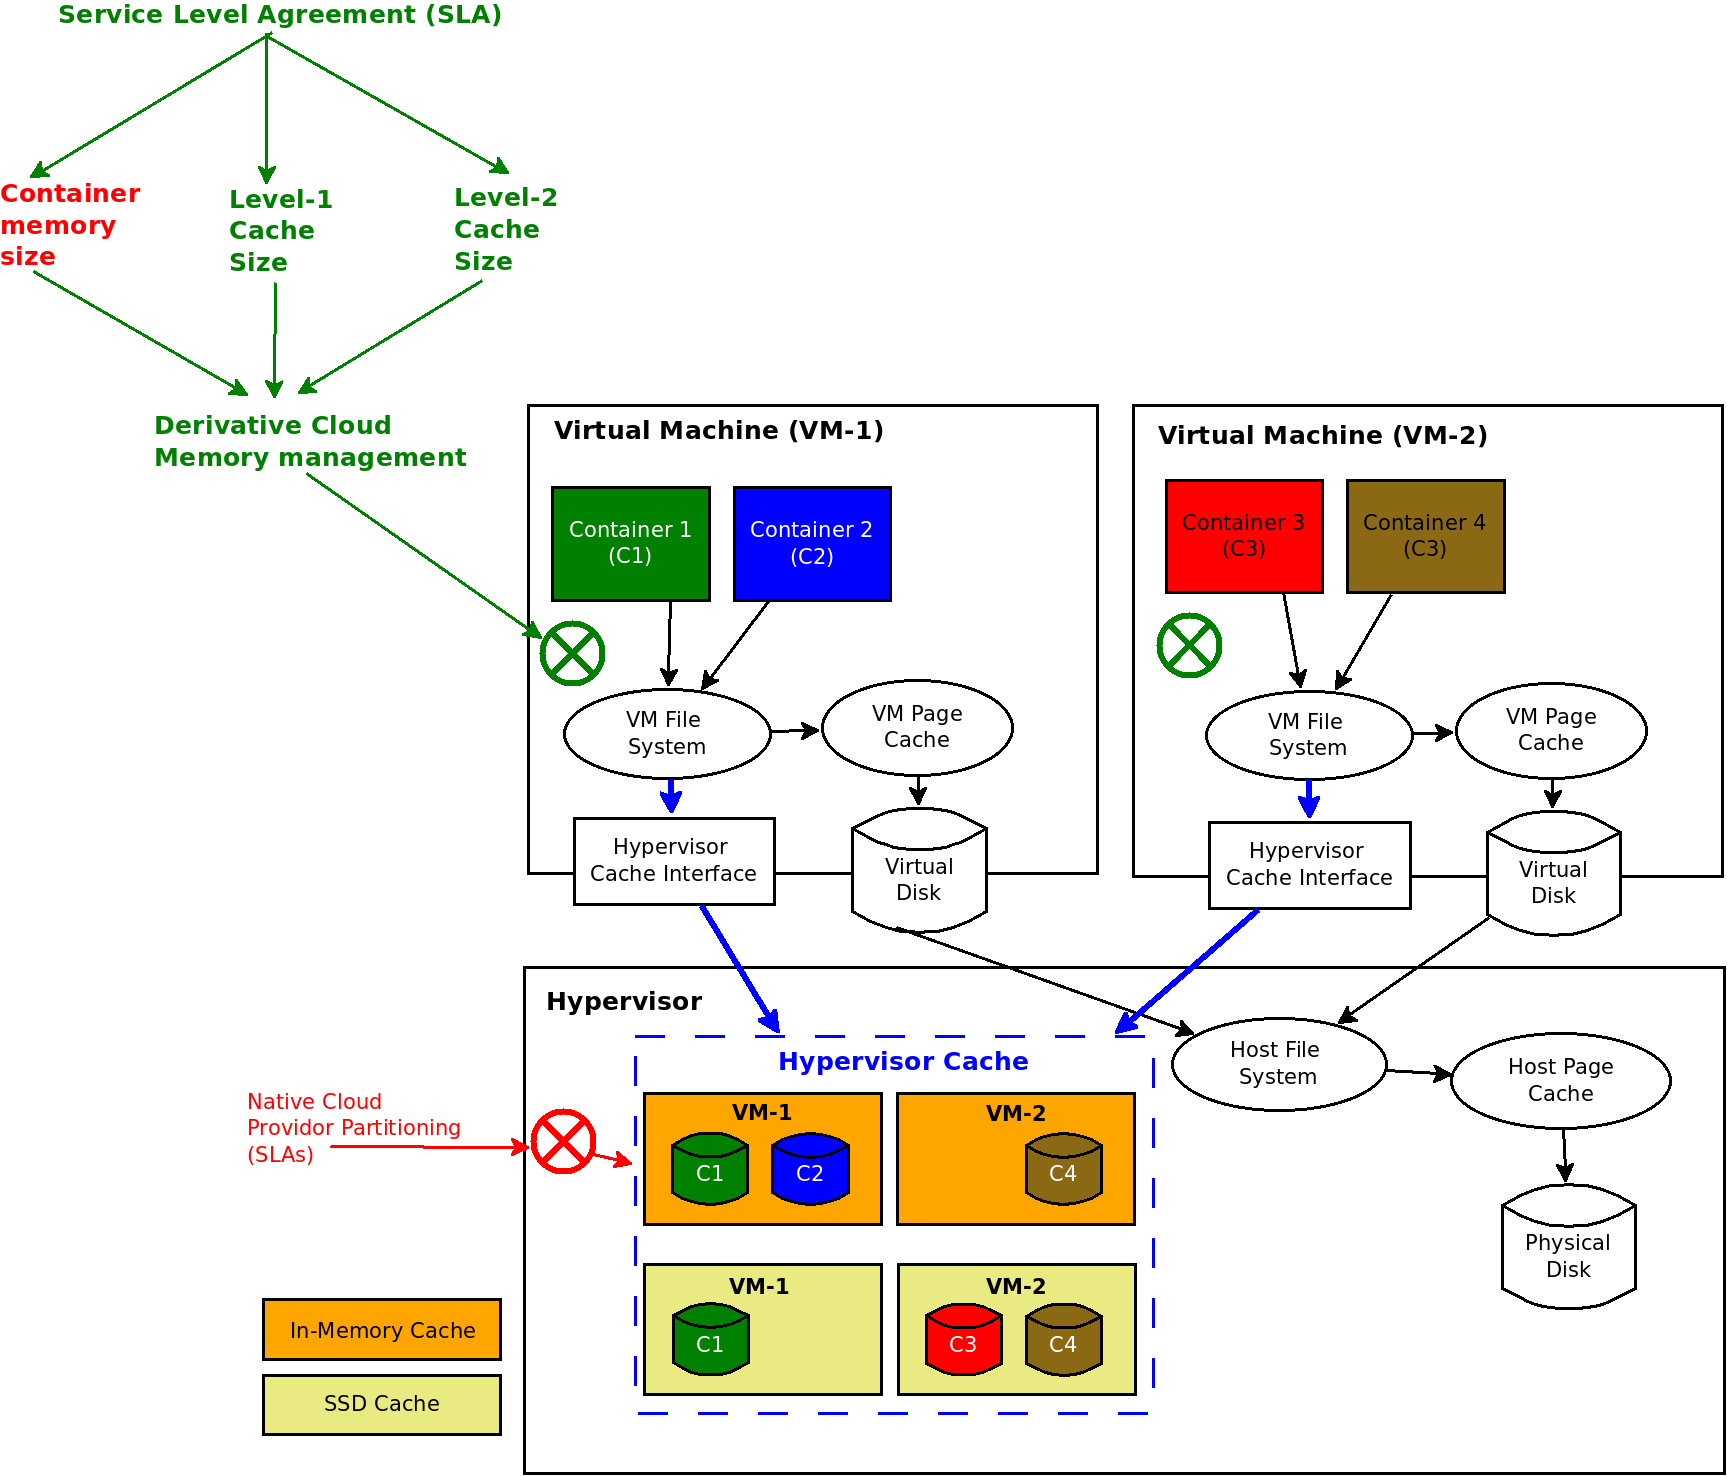
\includegraphics[scale=0.26]{/home/prashanth/Stage-2/Report/images/dd_design/architecture.png}
      \caption{Updated memory management framework}
      \label{plot:dd_architecture}
    \end{figure}
        
    \subsection{Decentralized memory management framework}
      Traditional caching frameworks and the earlier design of double decker centered around the idea 
      of a hypervisor managed cache with the hypervisor admin (native cloud provider) as the single sole 
      administrator of the system.
      
      We now propose a decentralized memory management framework with two control centers 
      who roles each have been discussed below. Most of the decision making is moved onto the
      derivative cloud provider sitting inside the virtual machine.
	      
      \subsubsection{Native provider cache partitioning framework}
	The native provider is now, only responsible for partitioning the caches for each VM
	based on its native cloud provider SLA. The native provider need not worry about 
	provisioning each of the container.

      \subsubsection{Derivative provider memory management framework}	
	The derivative provider is now responsible for managing three levels of memory entities,
	
	\begin{enumerate}
	  \item Container memory size
	  \item In-memory or level-1 cache
	  \item SSD or level-2 cache
	\end{enumerate}
	
	The derivative provider maps each application SLA onto a combination of these three management
	knobs to achieve desired application level objectives. This helps even provisioning of applications
	that cannot be helped by cache partitioning schemas, that is that they are anonymous memory dependent.


    \subsection{Hybrid cache}
      The hybrid cache is an updated version of the previous cache where each VM/container can be configured
      with a in-memory and SSD cache simultaneously. But with two-levels of caches configured to each application
      we need an mechanism to move objects (pages) of one level to another and vice-versa.
      
      Every PUT operation into the cache tries to first add the new object into the memory cache if configured, 
      and if not it adds it to the SSD cache.
      
      \subsubsection{Movement of objects}	
	There are two levels of cache movements, and have thresholds which trigger this movement. The movement of
	objects are described below. The thresholds and the eviction batches are all configurable.
	
	The level-1 and level-2 caches have a higher threshold after which objects are either \textit{demoted} to the 
	lower level (in the case of level-1, if level-2 is configured) or is evicted from the cache. Similarly
	there is also an lower-threshold at level-1 and when the cache occupied at level-1 is below the lower threshold
	and objects are present at level-2, objects are \textit{promoted} to level-1 is triggered.
	
	The target execution entity (VM/container) for promotions or demotions are purely based on the entities that
	are exceeding their allocations the most (or) most under-utilizing their allocations. The order for selection
	is VM is selected first, followed by the container.
      
	
  \section{Implementation specifics of the hybrid cache}

    The hybrid cache implementation is built upon the existing implementation of the double decker cache as described in 
    Section~\ref{sec:double_decker_internals}. Changes have been made to this implementation to accommodate the hybrid setup.
    
    \begin{figure}
      \centering
      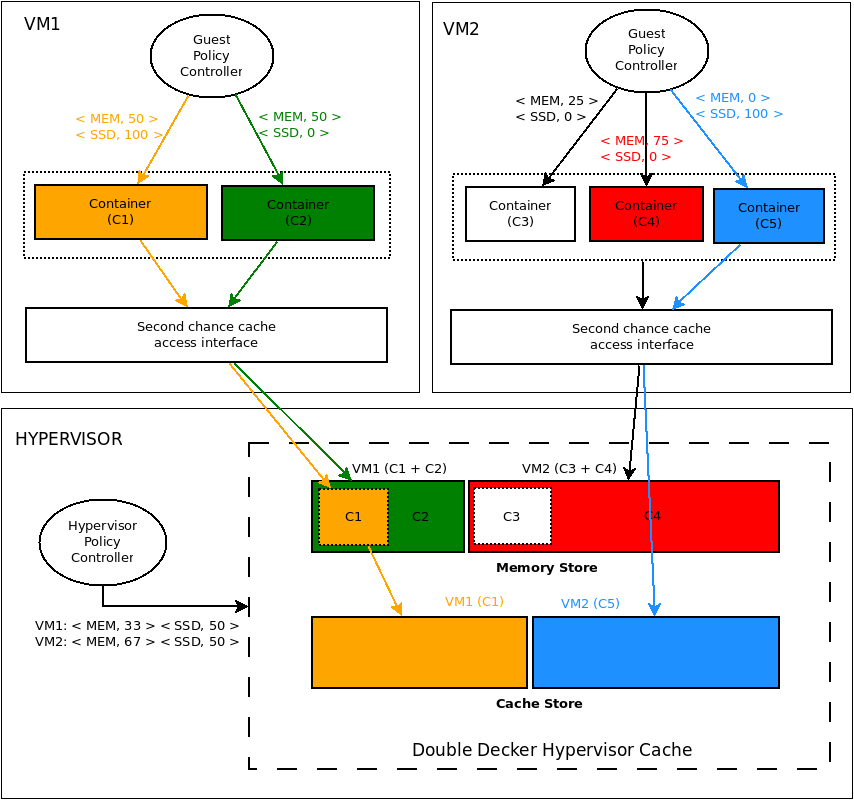
\includegraphics[width=0.75\textwidth]{/home/prashanth/Stage-2/Report/images/dd_design/implementation.png}
      \caption{\dd{} internals}
      \label{img:dd_internals}
    \end{figure}
  
      \subsubsection{Pool to accommodate both memory and SSD objects}
	The notion of pools as described in Section~\ref{sec:double_decker_internals} is carried over to the hybrid implementation.
	However, every pool for a particular container now contains a memory and SSD weight parameter. The VM also has a memory
	and SSD cache weight configuration parameter.
	
	The pool now stores both memory and SSD objects (as shown in Fig~\ref{img:dd_internals} using the same tree structure 
	that earlier stored a single type of object. The search mechanism is the same on the tree, but the tree node now either 
	points to a memory page or and SSD block based on the type of the node.  
	
	    
      \subsubsection{Asynchronous kernel threads for movement of objects}
	Two kernel threads were used to promote and demote objects between the two levels of cache. These kernel threads also
	performed eviction if movement of objects didn't clear up enough space. Asynchronous movement of threads required 
	proper synchronization and locking mechanisms to ensure consistency in data structure being manipulated. 
      
      \subsubsection{Multilevel stats}
	The stats that were earlier based on a single level, had to be changed to incorporate a multilevel stat. These 
	multilevel stats are developed to help provisioning of the three level knobs at the guest to satisfy application
	objectives.
  
  \section{Correctness of implementation}
  
      The experimental setup is just as described in Section~\ref{sec:dd_setup}.
      For establishing the correctness of our workload, we have considered a self 
      generated synthetic workload generated using \texttt{cat} command that 
      outputs the content of a file onto \texttt{/dev/null}. This workloads helps 
      us to validate the correctness of our implementation by predicting deterministic
      outputs.
  
    \subsection{Arithematic validation of stats}
    
      \myparagraph{Question}
	    To verify the correctness in accounting of stats while accessing cache at both levels.
	    
      \myparagraph{Procedure}
	We ran several experiments and computed the actual cache usage (memory and SSD) in our implementation. To an calculated 
	an estimated cache usage we used the formula given below. We used the same formula for both memory and SSD cache. 
	  \begin{equation}
	    EstimatedUsed = Puts + ObjectsMovedIn - (Gets + Flushes + ObjectsMovedOut)
	  \end{equation}
      
      \myparagraph{Observations}
	The values for \textit{EstimatedUsed} and \textit{ActualUsed} (present in out stat counter) matched in most cases.
	However, over long periods of run, with quite a large number of cache operations there was a marginal difference
	between the two (\textless 1\%).
	
      \myparagraph{Inference}
	Since the correctness of the actual value of cache used depend on the other stats that we have collected, and the 
	matching of \textit{EstimatedUsed} and \textit{ActualUsed} would only mean that all the stats collected are right.
    
    \subsection{Movement of objects between both levels of cache}
	
	To verify the correctness of our implementation empirically, we have taken our synthetic workload described in 
	above and ran a couple of simple experiments to demonstrate the expected 
	behavior of our cache to support cache operations like puts, gets, promotions and demotions.  
	
	\subsubsection{Memory to SSD cache}

	  \myparagraph{Question}
	    To verify the correctness in accounting of stats while accessing cache and moving objects from memory (L1) to SSD (L2) cache.
	    
	  \myparagraph{Procedure}
	      We start of the experiment with powering on the VM, followed by the container. We assigned complete memory and SSD cache 
	    at the double-decker back-end to support the container. The container had a \textbf{memory requirement of 2078 MB}, 2048 MB workload
	    requirement and 30 MB container requirement (container requirement was obtained by running the same experiment while having
	    a nearly 0 MB workload. The container was allocated with 2048 MB (512 MB of container memory + 512 MB of memory cache 
	    + 1024 MB of SSD cache). Now, the workload performed a sequential read of its workload (i.e 2048 MB) once.
	    Table~\ref{table:correctness_memtossd} shows the list of approx. estimated values (which are based on our 
	    implementation) and observed values for the metrics at the cache at the end of the experiment. 
	    
	    \vspace*{1em}	
	      \begin{table}
		\begin{center}
		  \begin{tabular}{ r | p{4cm} | p{4cm} }	      	    
			Metric & Approx. estimated Value & Observed Value \\ 
		    \hline
		    \hline
		    Puts (MB) & 2078 & 2080 \\
		    \hline
		    Gets (MB) & 0 & 1 \\
		    \hline
		    Container memory usage (MB) & 512 & 509 \\  
		    \hline
		    Memory cache usage (MB) & 504 & 503 \\
		    \hline 
		    SSD cache usage (MB) & 1008 & 1000 \\
		    \hline
		    Evicts (MB) & 54  & 64 \\
		    \hline
		    Flushes (MB) & 0  & 0 \\
		    \hline
		    Cumulative usage (MB) & 2078 & 2076 \\
		    \hline
		    Demotions (MB) & 1062 & 1064 \\
		    \hline
		    
		  \end{tabular}
		\caption{Comparison between expected and actual values}
		\label{table:correctness_memtossd}
		\end{center}	  
	      \end{table}
	    \vspace*{1em}
	    
	  \myparagraph{Observations}
	  The following are the observations,	  
	    \begin{enumerate}
	     \item There is a small number of gets, probably occurring due to pages used by other container applications.
	     \item Puts in the cache, is marginally (\textless2 MB) greater than expected value, and this deviation is due to the small number 
	     of Gets which are occurring.
	     \item The memory cache usage, is exactly as expected. However, SSD cache usage is slightly lesser than the expected value, 
	     but however the deviation seems to be an acceptable value.
	     \item The demotions (movement from memory to SSD) and cumulative usage values are nearly the same with a subtle deviation 
	     (\textless2 MB) which is an acceptable value.
	    \end{enumerate}

	  
	  \myparagraph{Inference}
	    The accounting stats, are nearly as expected. This verifies the correctness of most of the stats of our implementation (except promotions).
	    
	
	\subsubsection{SSD to memory cache}
	  
	  \myparagraph{Question}
	    To verify the correctness in accounting of stats while moving objects from SSD (L2) to memory (L1) cache.
	    
	  \myparagraph{Procedure}
	      We start of the experiment with powering on the VM, followed by the container. We assigned complete memory and SSD cache 
	    at the double-decker back-end to support the container. The container had a \textbf{memory requirement of 2078 MB}, 2048 MB workload
	    requirement and 30 MB container requirement (container requirement was obtained by running the same experiment while having
	    a nearly 0 MB workload. The container was allocated with 2560 MB (512 MB of container memory + 2048 MB of SSD cache).
	    The workload performed a sequential read of its workload (i.e 2048 MB) once, this lead to using up of nearly 1566 MB of SSD cache.
	    
	    Now, we changed the memory cache size to 256 MB while performing basic operations at the container which triggered the promotion 
	    (movement of objects from SSD to memory) of the objects to the memory cache. The promotion triggers all objects until the memory 
	    cache reaches a threshold usage - 192 MB in our case, as this threshold is calculated as,
	    
	    \begin{equation}
	      MemoryCacheLowerThreshold (192 MB) = MemoryLimit (256 MB) - LimitSize (64 MB)
	    \end{equation}
	    
	    Hence we would expect 192 MB worth of objects be promoted from SSD to memory cache in an ideal case.
	    
	    
	  \myparagraph{Observation}
	    Using our stats, it was observed that the estimated promotion and the actual promotion of objects were of an exact match with 
	    the number being 192 MB.
	    
	  \myparagraph{Inference}
	    This verifies the correctness in the accounting stats in movement of objects from SSD to memory cache. Hence movement 
	    of objects from both memory to SSD and vice-versa have been verified empirically.
  
  
  
  \section{Evaluation of Double Decker}
    Now, that we have established correctness of our implementation, we had put it to test its effectiveness in 
    tackling in previously mentioned drawbacks.
    
    %\subsection{Performance comparion with old implementation}
  
    \subsection{Provisioning for anonymous and file backed workloads}
      
    
    \subsection{Hybrid cache provisioning}
    
  %% \chapter{Implementation details}
% 
%   \section{Modified memory Cgroup}
%   
%     \subsection{Per container configurable weights}
%     
%     \subsection{Deterministic reclamation}
%     
%     \subsection{Flexible reclamation size}
%     
%   
%   \section{Double decker}
%   
%     \subsection{Existing memory management framework}
%     
%     \subsection{Updations to exisiting framework}
%     
%       \subsubsection{Multilevel configurable caches}
%       
%       \subsubsection{Asyncronous kernel threads for transfer of objects}
%       
%       \subsubsection{Multilevel stats}
%   
  %% 
% \chapter{Evaluation}
% 
%   \section{Updated memory Cgroup controller}
%   
%     \subsection{exp1}
%     \subsection{exp2}
%   
%   \section{Double decker}
%   
%     \subsection{exp1}
%     \subsection{exp2}
% 
%   
  
\chapter{Conclusions}
  
    We have made an initial attempt to understand memory management in Linux containers. We started off with purposing hypotheses based on 
theoretical evidences. We performed empirical analysis to verify the correctness of our purposed hypotheses. We also performed a few more 
empirical analysis to establish parts of memory management for which hypotheses couldn't be drawn. We then tried to extrapolate its 
implications in the real world applications running inside a derivative cloud environment. These implications strongly suggested that 
existing memory management techniques may impact higher provisioned containers negatively, when the system is under memory pressure. We 
conclude by purposing the requirements of a new desired policy that provides this notion of a differentiated reclamation to enforce 
deterministic allocation when the system is under memory pressure.  
  
 
  \chapter{Future Extensions}
  
    The following are the list of works that are to be taken up in the near future,
    
      \begin{enumerate}
	\item Design and implement a new memory management policy for containers.
	\item Analyze memory hierarchy in cgroups, and see how this affects containers.
	\item Explore other resource controller in the container framework, identify issues and provide appropriate fixes.
	\item The end goal is to provide an adaptive resource provisioning framework for containers. 
      \end{enumerate}

  

  
  \bibliographystyle{ieeetr}
  \bibliography{mylit}  
  
  %\appendix
  %\include{appendix/demos}
  %\include{appendix/benchmarks}

\end{document}

%%% Local Variables: 
%%% mode: latex
%%% TeX-master: t
%%% End: 
